\documentclass[12pt,a4paper]{article}
\usepackage[latin1]{inputenc}
\usepackage{float}
\usepackage{amsmath}
\usepackage{amsfonts}
\usepackage{amssymb}
\usepackage{graphicx}
\usepackage[hidelinks]{hyperref}
\usepackage{changepage}
\usepackage{subfig}
\usepackage{placeins}



\author{Davide Cocco - 944122\\
	Marco Gasperini - 944922}
\date{A.Y. 2019/2020 - Prof. Di Nitto Elisabetta}


\title{
	\textbf{\Huge{SafeStreets}} \\
	\large Requirements Analysis and Specification Document
}

\begin {document}

	\begin{figure}
		\centering
		
\includegraphics[width=1.0\linewidth]{Images/polimi.jpg}
	\end{figure}

	\maketitle
	\newpage
	\tableofcontents
	\newpage

\section{INTRODUCTION}
\subsection{Purpose} 
This document will contain the \texttt{Requirements Analysis and Specification Document} for SafeStreets, a crowd-sourced application that will allow users to notify traffic violations to authorities to assist them in law enforcement. Through a data mining system, authorities and their officers will receive relevant information in real time to help them with their job, and fining offenders will be accelerated through an automatic ticket emission functionality. The software will not be designed to substitute the existing system, but rather to improve its efficiency.
 
\subsection{Scope}
The software will be dedicated to civilians and authorities: through a mobile application, civilians will have the possibility to report a violation by submitting pictures, position, date and the license plate of the offender to the authorities in an effort to improve their communities, while officers can use the data mining system, which updates a map periodically with new reports and highlights areas with high violation frequency, to facilitate the process of law enforcement by locating offences and releasing tickets. Authorities will be supplied with a web application with the ability to add new officers, and will also have access to the aforementioned system.
A data warehouse will be thus implemented, and repeated reports of violations could also lead to automated traffic tickets being released at the discretion of the authorities.
The system will be designed to avoid any kind of voluntary or unpredictable behaviour which may result in invalid reports or wrong fines being released, with a vigorous effort to completely prevent harmful usage of the S2B rather than correcting it a posteriori.
\newpage
\subsubsection{Phenomena table}
\FloatBarrier
\begin{center}
\begin{table}[h]
    \begin{tabular}{|l|c|c|}
    	  \hline
      \textbf{Phenomenon} & \textbf{Shared} & \textbf{Who controls it?} \\ \hline
	  Occurrency of traffic violation & No & World \\
	  Filing a violation report & Yes & World \\
	  Registration and login of any type of user & Yes & World \\
	  Selection of correct or wrong reports made by authority & Yes & World \\
	  Arrival of an officer at the site of the violation  & No & World \\
	  Confirmation or rejection of a report by the officer & Yes & World \\
 	  Requesting of bans & Yes & World \\
	  Creation of reports composed by photo, date and location & No & Machine \\
	  Creation of traffic tickets & No & Machine \\
	  Collection and processing of data & No & Machine \\
	  Presentation of relevant data about violations and offenders & Yes & Machine \\
	  Issuing of bans & Yes & Machine \\
	  Officer corfirming the checking of a report & Yes & Machine \\ \hline
    \end{tabular}
\end{table}
\end{center}
\FloatBarrier
\subsubsection{Goals}
\begin{itemize}
\item {\textbf[}\textbf{G1}{\textbf]}: Allow future users to easily register and login. 
\item {\textbf[}\textbf{G2}{\textbf]}: Allow users to notify authorities of traffic violations through the use of the camera.
\item {\textbf[}\textbf{G3}{\textbf]}: Store relevant info about the violation in the data warehouse.
\item {\textbf[}\textbf{G4}{\textbf]}: Assist authorities in the process of law enforcement:
\begin{itemize}
	 \item {\textbf[}\textbf{G4.1}{\textbf]}: allow automatic ticket compilation at the discretion of the authorities;
	\item {\textbf[}\textbf{G4.2}{\textbf]}: show processed data relevant to the purpose.
\end{itemize}
\item {\textbf[}\textbf{G5}{\textbf]}: Guarantee security: 
\begin{itemize}
	\item {\textbf[}\textbf{G5.1}{\textbf]}: allow discarding of invalid reports;
	\item {\textbf[}\textbf{G5.2}{\textbf]}: avoid unauthentic officer registrations by design;
	\item {\textbf[}\textbf{G5.3}{\textbf]}: block people who came in possession of an officer's device to cause any damage;
	\item {\textbf[}\textbf{G5.4}{\textbf]}: ban users who abuse of the violation reporting system.
\end{itemize}
\item {\textbf[}\textbf{G6}{\textbf]}: Guarantee privacy to users.
	\begin{itemize}
	\item {\textbf[}\textbf{G6.1}{\textbf]}: only allow authorities to visualize relevant data for law enforcement purposes.
	\end{itemize}
\end{itemize}
\subsection{Definitions,	Acronyms,	Abbreviations} 
\subsubsection{Definitions}
 \begin{itemize}
\item \texttt{Violation | Offence:} we will strictly refer to any kind of static traffic violation, especially parking violations. 
\item \texttt{Authority:} a law enforcement authority which is manages traffic violations, it could be the local police, the traffic wardens etc. We will refer with this term also to the personnel which operates the web application in the authorities' headquarters.
\item \texttt{User:} refers to the users of the mobile application, that is officers and civilians.
\end{itemize}
\subsubsection{Acronyms}
\begin{itemize}
\item \texttt{S2B:} software to be.
\item \texttt{HFVZ:} high violation frequency zone.
\item \texttt{GPS:} Global Positioning System.
\item \texttt{GDPR:} General Data Protection Regulation.
\item \texttt{DW:} data warehouse.
\item \texttt{VLA:} Vehicle Licensing Authority.
\end{itemize}
\subsubsection{Abbreviations}
\begin{itemize}
				\item {[Gn]}: n-goal.
				\item {[Rn]}: n-requirment.
				\item {[Dn]}: n-domain assumption
				\item {App}: application.
			\end{itemize}
\subsection{Revision history} 
\subsection{Reference	Documents} 
\begin{itemize}
				\item Specification Document "Mandatory Project Assignment A.Y. 2019/2020"
				\item 830-1993 - IEEE Recommended Practice for Software Requirements
				\item "Appunti di Sistemi Informativi per il Settore dell'Informazione" A.Y. 2018/2019
				\item Alloy Language Reference "http://alloytools.org/download/alloy-language-reference.pdf"
				\item UML diagrams: https://www.uml-­diagrams.org/
			\end{itemize}
\subsection{Document	Structure} 
\begin{enumerate}
			\item \texttt{Introduction}: the first section is a general description of the system's scope and its goals. It also includes the revision history of the document and its references. Definitions and abbreviations used along the paper will be provided.
			\item \texttt{Overall Description}: this section includes shared phenomena, requirements and domain assumptions. It also clarifies users' needs.
			\item \texttt{Specific Requirements}: this section includes all the requirements, both functional and non functional.
			\item \texttt{Formal Analysis Using Alloy}: it includes the Alloy model of the described system.
			\item \texttt{Effort Spent}: this section includes information about the hours spent to compile this document.
			\item \texttt{References}: this section includes references about papers/documents used to support this document.
		\end{enumerate}
\newpage
\section{OVERALL	DESCRIPTION}
\subsection{Product	perspective} 
This class diagram shows a bird's eye view of the system:
\begin{figure}[H]
				\centering
					\begin{adjustwidth}{-25mm}{-25mm}
					        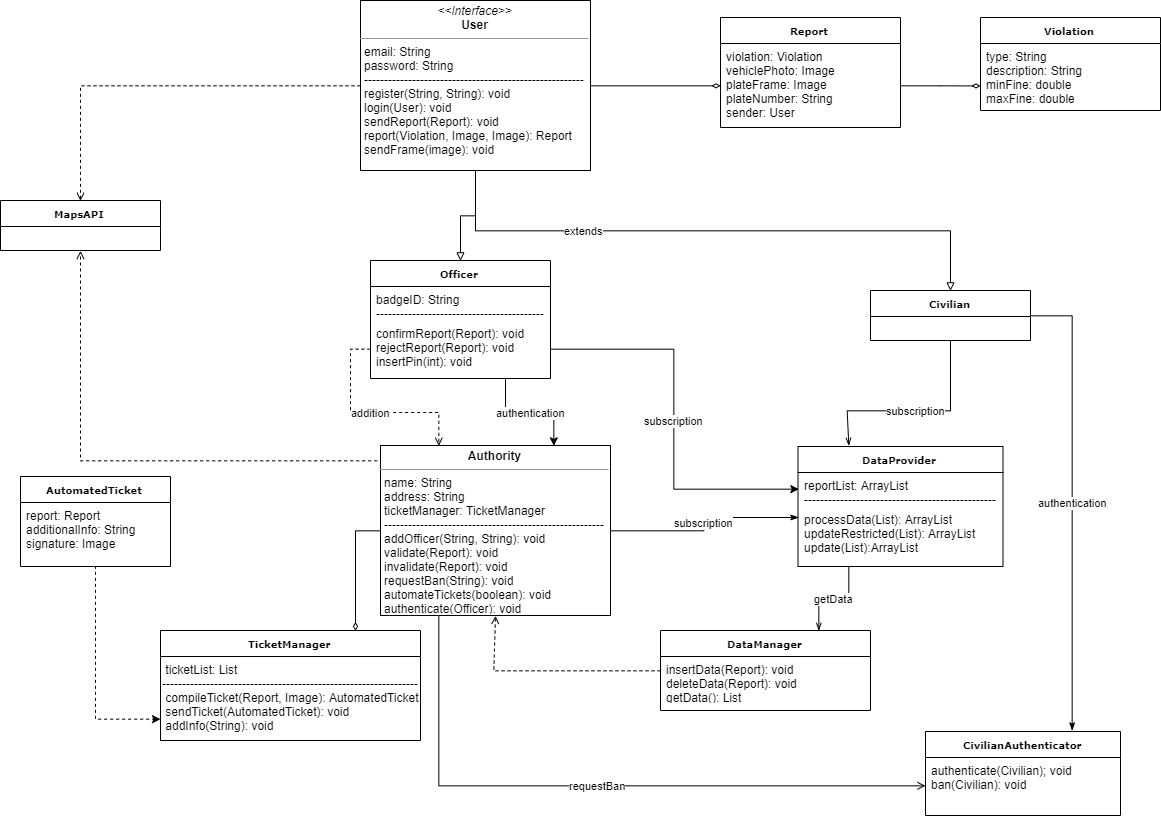
\includegraphics[width=.9\paperwidth,keepaspectratio]{Images/class_diagram}
					\end{adjustwidth}
				\label{fig:automated_request_sequence}
			\end{figure}
\newpage
These state diagrams describe the possibilities of each actor and how their bevahiour will be influenced by the system and externl factors.
	\subsection{Civilian}
			\begin{figure}[H]
				\centering
					\begin{adjustwidth}{-25mm}{-25mm}
					        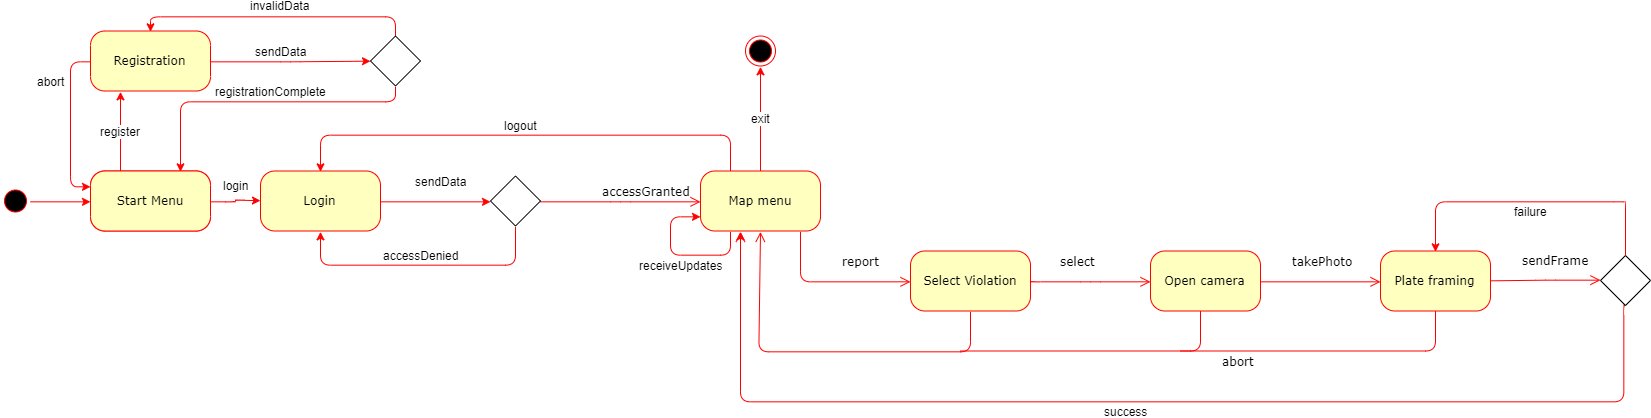
\includegraphics[width=.9\paperwidth,keepaspectratio]{Images/civilian_states}
					\end{adjustwidth}
				\label{fig:automated_request_sequence}
			\end{figure}
	\subsection{Officer}
			\begin{figure}[H]
				\centering
				\begin{adjustwidth}{-25mm}{-25mm}
					        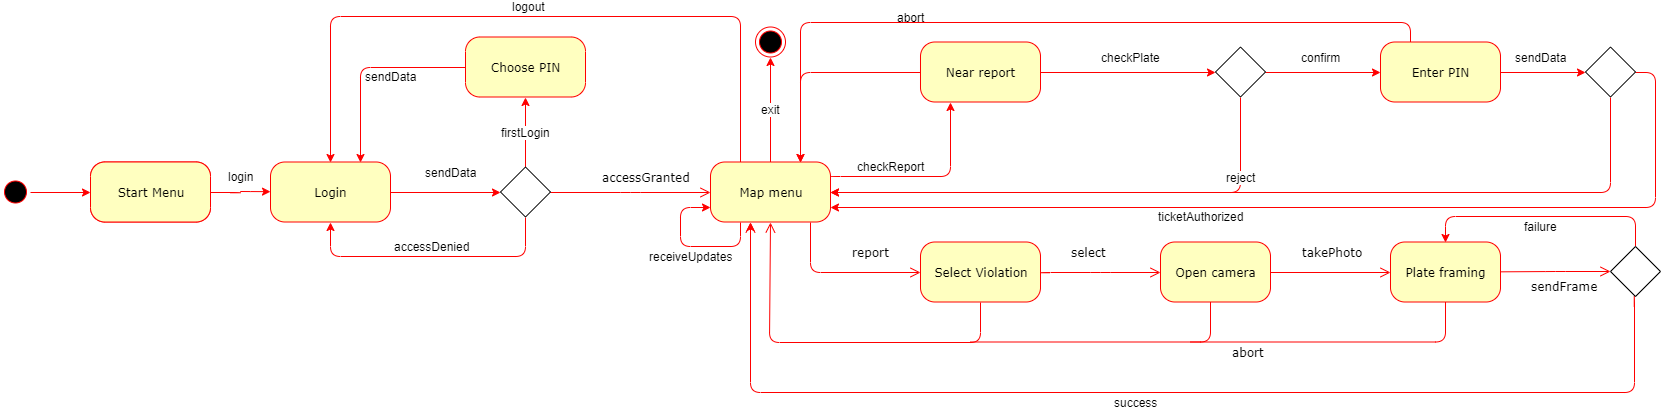
\includegraphics[width=.9\paperwidth,keepaspectratio]{Images/officer_states}
					\end{adjustwidth}
				\label{fig:automated_request_sequence}
			\end{figure}
	\subsection{Authority}
			\begin{figure}[H]
				\centering
				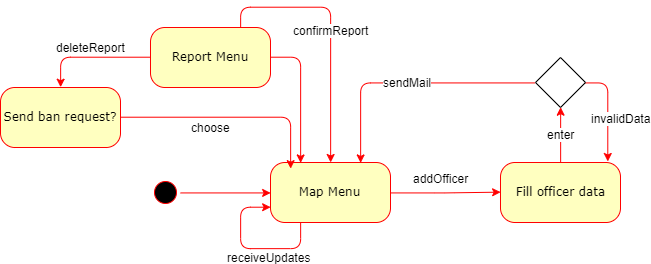
\includegraphics[width=.9\textwidth,keepaspectratio]{Images/authority_states}
				\label{fig:automated_request_sequence}
			\end{figure}
\subsection{Product	functions}
The goals to be accomplished require the following functions:
 \begin{itemize}
\item \texttt{Registration and login management:} while civilians will be able to register and login in standard fashion through email and password, officers will be added by authorities through their client: an automatically generated password will be sent to their email, and they will be able to access through their badge ID and such password. This way it is impossible for civilians to log in as an officer, as they would have to know both the badge number and the password contained in the officer's personal email.

\item \texttt{Violation reporting:} allow users (both civilians and officers) to choose between a set of offences and send various pictures representing it, with the corresponding date and location (via GPS and system timestamping) to the authority which will process them and discard incoherent or wrong ones. Photos can only be taken in real time and not uploaded to avoid manipulations.

\item \texttt{Ban requesting:} if authorities receive undescriptive photos or in any shape or form useless reports, they can send a request from the authorities' client to the SafeStreets HQ's server to ban the abusing user.

\item  \texttt{Data storage, mining and visualization:} store all the relevent data from the reporting procedure to process it through ETL and present it to the authority to assist them in law enforcement. The most important functionality will be periodically updating the map in the officers' and authorities' GUIs with new violations and hightlightings of HVFZs, and also listing repetead offenders. 

\item  \texttt{Automated ticket emission:} officers can locate violations through the map, and through a unique code sent to the authority, sign an automatically compilated ticket which will be emitted and sent via email to the Vehicle Licensing Agency. The code is to make sure that even if the officer's mobile is stolen while he's logged in, the thief cannot emit tickets.
\end{itemize}
\newpage
\subsection{User characteristics}
 \begin{itemize}
\item \texttt{Visitors:} users who haven't yet registered or logged in the mobile application, they are only able to register as a civilian or log as a civilian (through email and password) or as an officer (through Badge ID and password issued by the authority). They interact with:
		\begin{itemize}
			\item Registration and login management.
		\end{itemize}

\item \texttt{Civilians:} users unaffiliated to law enforcement authorities who are interested in improving their community, they are only able to report violations but don't have access to mined data (except the updated map with HVFZs). They're required to be registered and log in the mobile application so they can eventually be excluded in case of security violations. They interact with: 
		\begin{itemize}
			\item Registration and login management;
			\item Violation reporting;
			\item Data storage, mining and visualization: only the map with HFVZ highlightings.
		\end{itemize}
 
\item \texttt{Officers:} they're registered to the mobile application through their authority listing by their badge ID them through the web application and receiving a password. They're able to see the mined data, report violations, and sign the automated tickets.  They interact with: 
		\begin{itemize}
			\item Registration and login management;
			\item Violation reporting;
			\item Data storage, mining and visualization;
			\item Automated ticket emission.
		\end{itemize}

\item \texttt{Users:} we will use this name only as a general way to refer to both registered officers and civilians when we're describing actions they are both able to perform in the same way (like compiling violation reports).

\item  \texttt{Authorities:} they're manually registered by SafeStreets personnel, and their work is managed in office by an officer using the SafeStreets web application. They can add new officers or confirm self-registered ones, and they're able to see the processed data, enable automatic ticket emissions, receive violation reports and thus discriminate between valid and invalid ones. They can request bans which the SafeStreets server will take care of issuing and can see every officer connected to the application. They interact with: 
		\begin{itemize}
			\item Violation reporting;
			\item Data storage, mining and visualization;
			\item Automated ticket emission;
			\item Ban requesting.
		\end{itemize}

\end{itemize}
\subsection{Domain assumptions} 
\begin{itemize}
\item {\textbf[}\textbf{D1}{\textbf]}: The officer's Badge ID is assumed to be unique.
\item {\textbf[}\textbf{D2}{\textbf]}: Users are assumed to provide a valid email.
\item {\textbf[}\textbf{D3}{\textbf]}: At least one of the city's authorities' server is always online to process reports and officer logins.
\item {\textbf[}\textbf{D4}{\textbf]}: Users' devices support the Mobile Application 
\item {\textbf[}\textbf{D5}{\textbf]}: Users' devices camera and GPS work correctly.
\item {\textbf[}\textbf{D6}{\textbf]}: Email from SafeStreets containing the confirmation link for registration is always received correctly.
\item {\textbf[}\textbf{D7}{\textbf]}: Email from the authority containing the officer's password is always received correctly.
\item {\textbf[}\textbf{D8}{\textbf]}: Authorities' devices support the web application.
\item {\textbf[}\textbf{D9}{\textbf]}: Authorities correctly receive the great majority of reports.
\item {\textbf[}\textbf{D10}{\textbf]}: The web application at the authorities' location is operated by an assigned officer most of the time.
\item {\textbf[}\textbf{D11}{\textbf]}: Officers only sign correct tickets and always check the license plate matches with the reported one.
\item {\textbf[}\textbf{D12}{\textbf]}: Location is calculated correctly by the device with at most 5 meters range from the user's position.
\item {\textbf[}\textbf{D13}{\textbf]}: Only the officer knows his personal pin that allows him to proceed in ticket compilation.
\item {\textbf[}\textbf{D14}{\textbf]}: The personnel operating the Authority's client discards most of the invalid reports.
\item {\textbf[}\textbf{D15}{\textbf]}: Every registered officer's signature is stored at the authority in an image file.
\end{itemize}
\section{SPECIFIC	REQUIREMENTS}
\subsection{External	Interface	Requirements} 
\subsubsection{User	Interfaces}
The following mockups give a basic idea of how the Mobile Application and the Web Application are supposed to look like.
\begin {itemize}
	\item \textbf{Users}: they can access to SafeStreets functionalities through the smartphone application.					
		\begin{figure}[H]
			\centering
			\subfloat [][\emph {Main Page}]
			{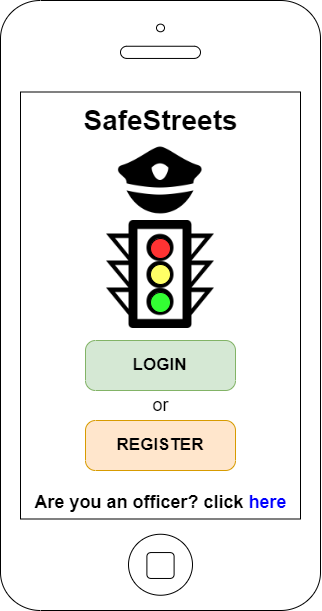
\includegraphics[width=0.3\linewidth]{Images/Mockup/SchermataIniziale.png}}\quad
			\subfloat [][\emph {Login}]
			{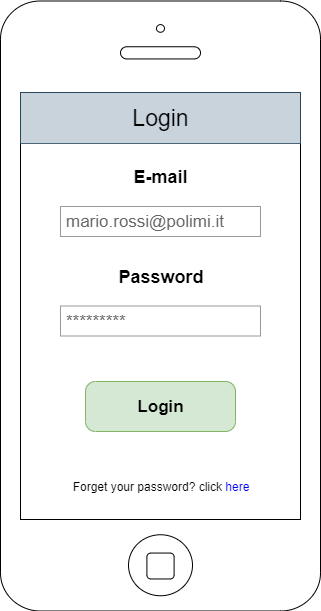
\includegraphics[width=0.3\linewidth]{Images/Mockup/Login.png}}\quad
			\subfloat [][\emph {Data update}]
			{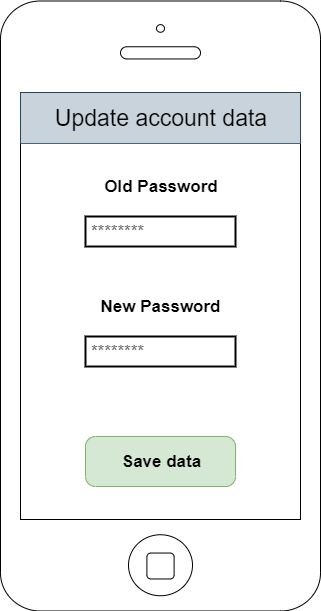
\includegraphics[width=0.3\linewidth]{Images/Mockup/UpdateData.png}}
			\caption{Login, Registration}
		\end{figure}
		\begin{figure}[H]
			\centering
			\subfloat [][\emph {Main menu}]
			{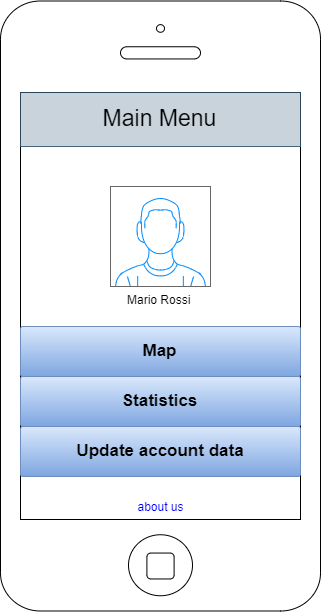
\includegraphics[width=0.3\linewidth]{Images/Mockup/user/User_Menu.png}}\quad
			\subfloat [][\emph {Statistics menu}]
			{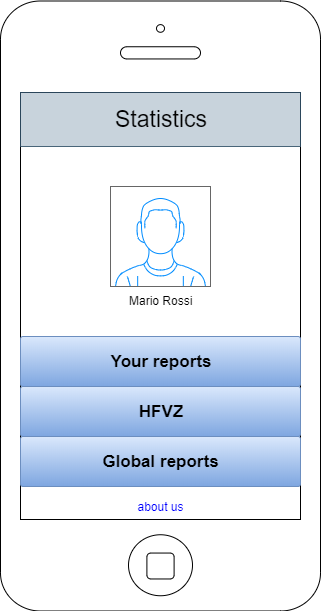
\includegraphics[width=0.3\linewidth]{Images/Mockup/user/UserStatisticsMenu.png}}
			\caption{User's Menu}
		\end{figure}
		\begin{figure}[H]
			\centering
			\subfloat [][\emph {Your reports}]
			{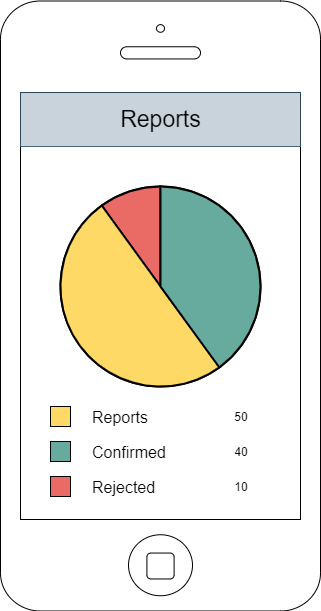
\includegraphics[width=0.3\linewidth]{Images/Mockup/user/UserStatistics_Reports.png}}\quad
			\subfloat [][\emph {HFWZ}]
			{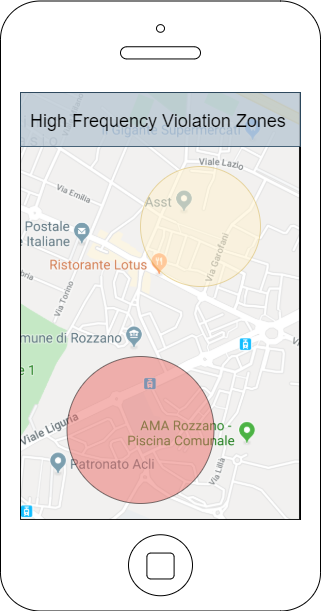
\includegraphics[width=0.3\linewidth]{Images/Mockup/Statistics_HFVZ.png}}\quad
			\subfloat [][\emph {Global Reports}]
			{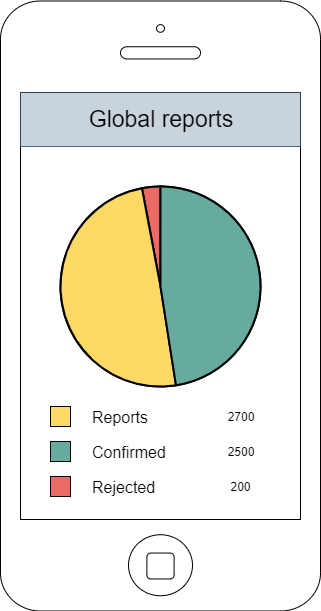
\includegraphics[width=0.3\linewidth]{Images/Mockup/Statistics_GlobalReports.png}}	
			\caption{User's Statistics}
		\end{figure}
		\begin{figure}[H]
			\centering
			\subfloat [][\emph {View report}]
			{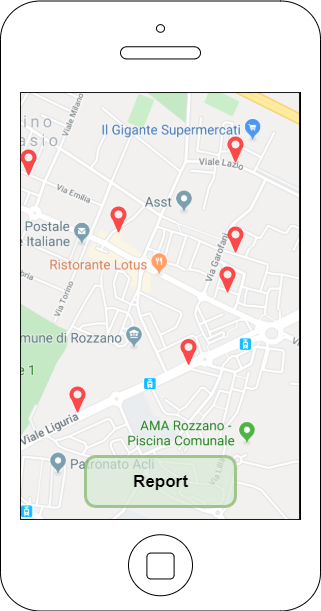
\includegraphics[width=0.3\linewidth]{Images/Mockup/Report.png}}\quad
			\subfloat [][\emph {Make report}]
			{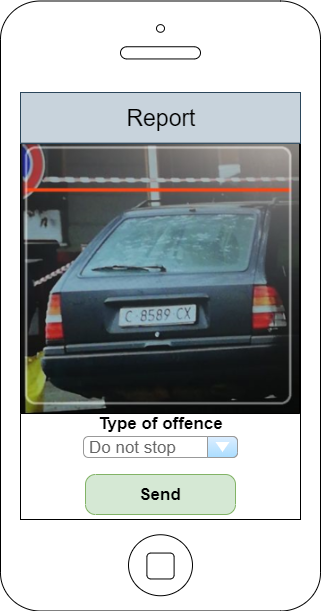
\includegraphics[width=0.3\linewidth]{Images/Mockup/user/ReportPhoto.png}}
			\caption{Report}
		\end{figure}
	\item \textbf {Officer}: They can investigate the reports and sign automated tickets.
		\begin{figure}[H]
			\centering
			\subfloat [][\emph {Main Page}]
			{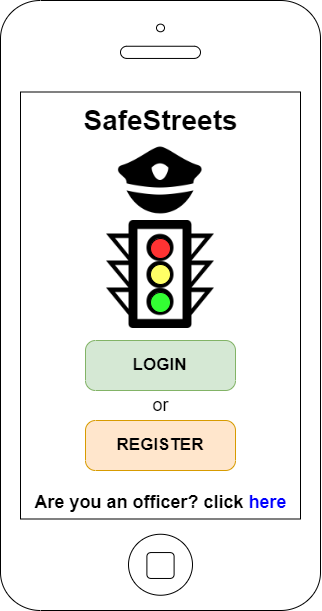
\includegraphics[width=0.3\linewidth]{Images/Mockup/SchermataIniziale.png}}\quad
			\subfloat [][\emph {Login}]
			{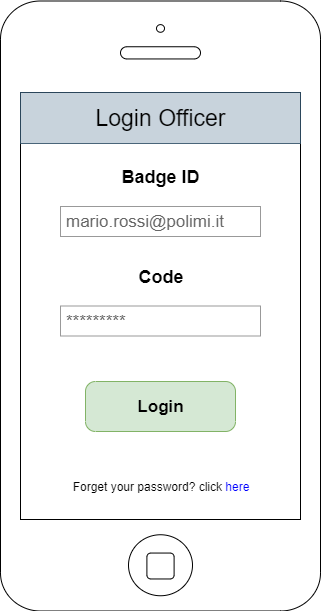
\includegraphics[width=0.3\linewidth]{Images/Mockup/officer/LoginOfficer.png}}\quad
			\subfloat [][\emph {Officer PIN}]
			{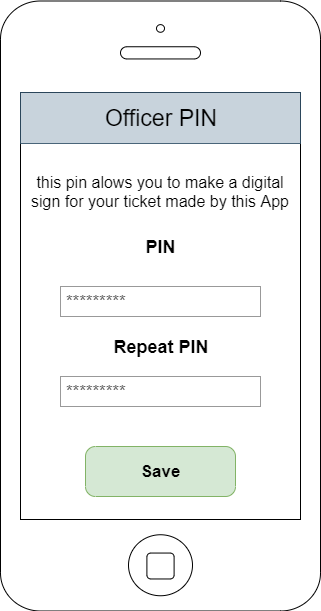
\includegraphics[width=0.3\linewidth]{Images/Mockup/officer/OfficerPIN.png}}
			\caption{Login, Registration, PIN}
		\end{figure}
		\begin{figure}[H]
			\centering
			\subfloat [][\emph {Main menu}]
			{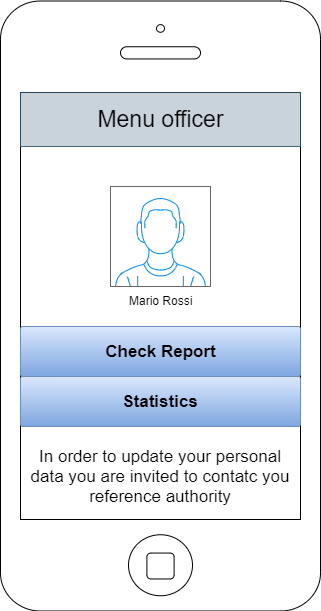
\includegraphics[width=0.3\linewidth]{Images/Mockup/officer/MenuOfficer.png}}\quad
			\subfloat [][\emph {Statistics menu}]
			{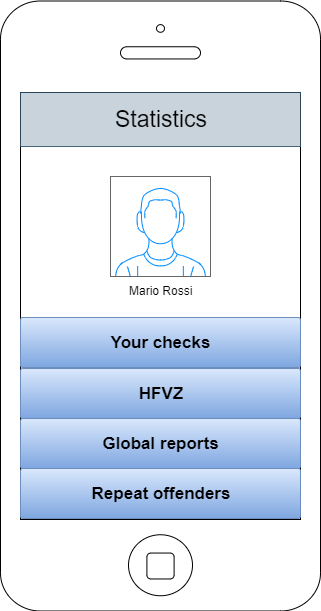
\includegraphics[width=0.3\linewidth]{Images/Mockup/officer/OfficerStatisticsMenu.png}}
			\caption{Officer's Menu}
		\end{figure}
		\begin{figure}[H]
			\centering
			\subfloat [][\emph {Your checks}]
			{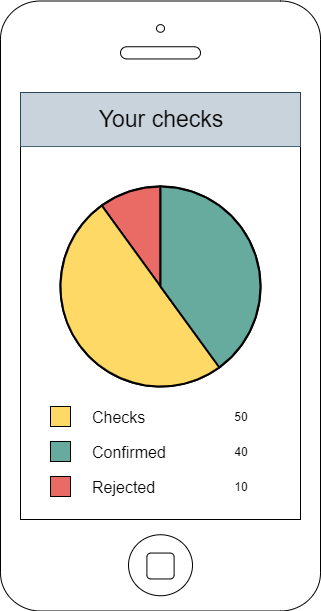
\includegraphics[width=0.3\linewidth]{Images/Mockup/officer/OfficerStatistics_YourChecks.png}}\quad
			\subfloat [][\emph {HFWZ}]
			{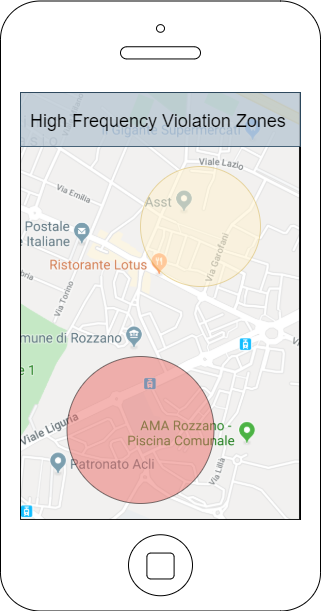
\includegraphics[width=0.3\linewidth]{Images/Mockup/Statistics_HFVZ.png}}
		\end{figure}
		\begin{figure}[H]
			\centering
			\subfloat [][\emph {Global Reports}]
			{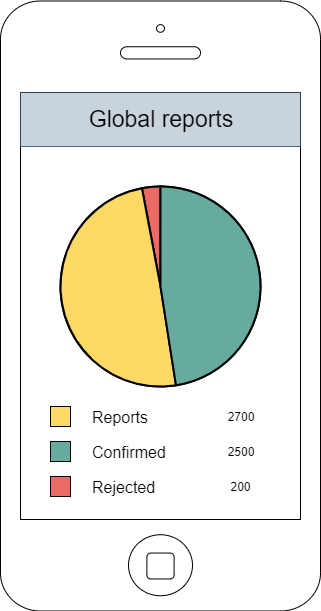
\includegraphics[width=0.3\linewidth]{Images/Mockup/Statistics_GlobalReports.png}}\quad
			\subfloat [][\emph {Repeat Offenders}]
			{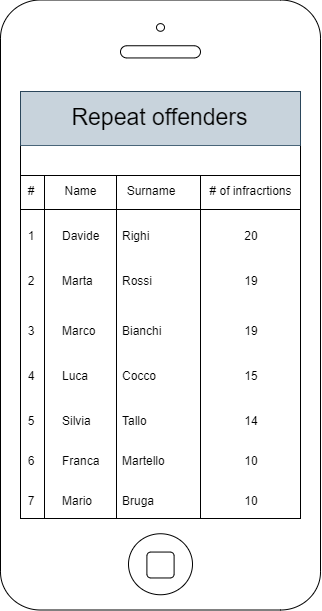
\includegraphics[width=0.3\linewidth]{Images/Mockup/officer/Statistics_RepeatViolations.png}}
			\caption{Officer's Statistics}
		\end{figure}
		\begin{figure}[H]
			\centering
			\subfloat [][\emph {Check violation}]
			{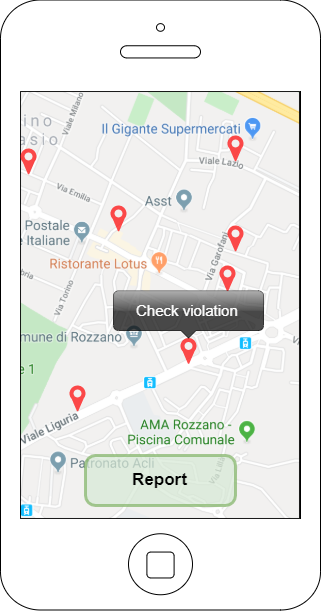
\includegraphics[width=0.3\linewidth]{Images/Mockup/officer/CheckViolation.png}}\quad
			\subfloat [][\emph {Under investigation}]
			{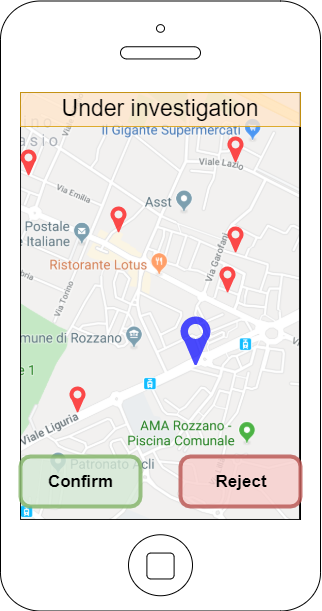
\includegraphics[width=0.3\linewidth]{Images/Mockup/officer/UnderInvestigation.png}}
		\end{figure}
		\begin{figure}[H]
			\centering
			\subfloat [][\emph {Violation confirmed}]
			{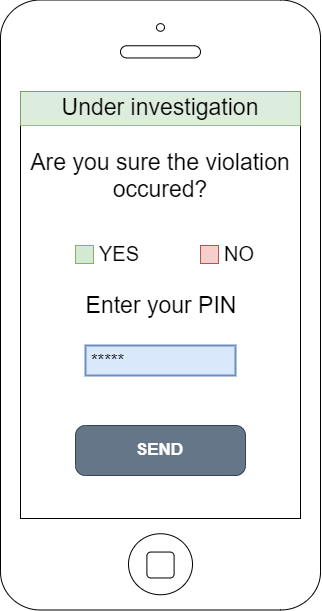
\includegraphics[width=0.3\linewidth]{Images/Mockup/officer/ViolationConfirmed.png}}\quad
			\subfloat [][\emph {Violation Rejected}]
			{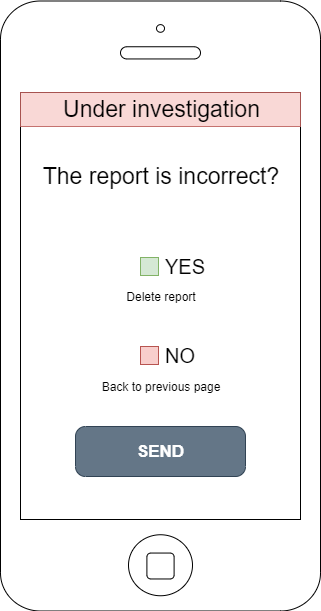
\includegraphics[width=0.3\linewidth]{Images/Mockup/officer/ViolationNotConfirmed.png}}
			\caption{Investigation}
		\end{figure}
	\item \textbf{Authority}: SafeStreets provides a Web Application for law enforcement authorities where they can validate reports, request bans, toggle the automated ticket emission functionalities on or off, and most importantly add new officers.
		\begin{figure}[H]
			\centering
			{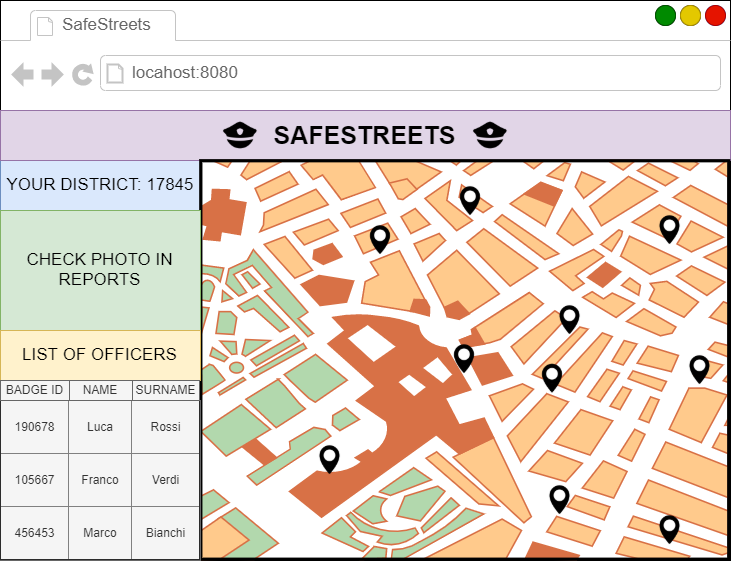
\includegraphics[width=1\linewidth, height=.5\linewidth]{Images/Mockup/AuthorityWebApp.png}}
			\caption{Web App}
		\end{figure}
\end{itemize}
\subsubsection{Hardware	Interfaces}
Since the application must run over the Internet, all the hardware shall require to connect network will be an hardware interface for the system, both
server and client side.
\begin{itemize}
\item Server-side: e.g. Modem, WAN - LAN, Ethernet Cross-Cable.
\item Client-side: e.g. Wi-Fi 802.11ac+ antenna, 3G/4G antenna. 
\end{itemize}
\subsubsection{Software	Interfaces}
SafeStreets will provide a very basic API for authorities to customize data about tickets and fines (so that the functionality can fit various legislations) and other minor parameters such as report expiration time.
The \texttt{Google Maps API} will be used to implement the map and geolocalization services.
\subsubsection{Communication	Interfaces}
HTTP will be used for communication between the nodes of the network along with the most recent TLS version to secure messages containing sensitive data. 
\subsection{Scenarios}
This section describes some of the scenarios in which SafeStreets may be used. Scenarios omit steps already described in previous ones: 

\subsubsection{User registration}
Giancarlo saw the advertisement of SafeStreets and decided to download the mobile application to report a car that always parks on the sidewalk outside his house and blocks the passage of pedestrians. After downloading and launching the new app, he is asked to fill a registration form in which he must insert his email address and a password. After clicking the "Sign In" button he receives an email with a link to confirm his registration, which he clicks to finalize his registration. From now on he can login and report offences with the "Report" button in the main screen.

\subsubsection{Correct violation reporting}
Mary just logged in as a civilian to report a double-parked car. Since it's her first use of the application, she's asked to allow SafeStreets to access her GPS and camera, to which she complies. She clicks "Report" on his main screen and chooses a violation from the modal which pops up. The app then opens her camera asking to take a photo of the vehicle showing the offence being committed. Then she's asked to frame the license plate with her camera, and the supervised learning algorithm scans the various frames looking for an interpretation for the image. The app then associates the report with a timestamp and a GPS position, and sends it to one of the authorities' servers. After a couple of minutes, Mary receives a notification informing her her report was correctly accepted and processed.

\subsubsection{Wrong violation reporting}
Simon decides to use the app to report his neighbour's vehicle because he doesn't like him. He sends a photo which in fact doesn't show any violation being committed. Arthur, a policeman who's working with the SafeStreets web application at his barracks, receives the report and notices there's clearly no violation being committed in the photo, and clicks on the "Warn" button which alerts the SafeStreets server of an invalid report, and discards the report immediately after. After a couple of minutes, Simon receives a notification telling him he's been forbidden from using the reporting function for a month.

\subsubsection{Officer registration}
Billy is a policeman whose barrack has just installed the SafeStreets application and data server. He received an email notifying him that he may be enabled to utilize the service. After a while, he receives an email from his barrack's SafeStreet client containing an automatically generated code. By entering his badge ID and this code in the officer login section of the mobile application, Billy is now able to login when he desires by using the code as password. Once logged in, Billy will have to enter a 5-digit pin that will allow him to make a traffic ticket signed by him when he receives a report.
Bill now sees the map of his surroundings, periodically updated with new traffic offence reports and with HFVZ highlighted. 

\subsubsection{Correct Ticket Emission}
John was on patrol this morning and checked on the SafeStreets App if there was any report in his vicinity. As soon as he logged in he noticed a reported violation in the map, about 250 meters from his position. John clicks the "Accept" button on the tooltip to confirm to other active officers he's checking the authenticity of the violation, and avoiding any other one of replicating this task. He now sees the photos of the reporting and the type of offence. Once he's near the vehicle, a "Confirm" button pops up. John checks that the vehicle is effectively committing a violation and the license plate matches the one in his screen. Once John clicks it and enters his secret 5 digit pin his authority's server will be able to place his signature into an automatically generated ticket that will be sent to the Vehicle Licensing Authority. Now the violation tooltip can disappear and John goes on with his duties.

\subsubsection{Wrong report discarded by an officer}
Gabriele, who is an officer, is walking towards an offence reported from SafeStreets. As soon as he arrives there, he realizes that the report involved a car parked on the pedestrian crossing which is no longer there. So he decides to click on the "Delete" button which subsequently communicates to the authority's server to remove it from the map.

\subsection{Requirements}
Here we include a list of both functional and non-functional requirements which will allow the efforts of the team to be concretely directed to the goals.
\subsubsection{G1: Allow future users to easily register and login.}
	
	\begin{itemize}
			\item \textbf{R1}: Separate civilian and officer registration and login functionality;
			\item \textbf{R2}: Data has to be correctly queried server-side everytime, to make sure no duplicate accounts are created or no unregistered visitors log in;
			\item \textbf{R3}: Send confirmation emails within at most one minute after the registration confirmation receipt (or the new officer being added); 
			\item \textbf{R4}: Confirm user registration within at most one minute after the email link has been clicked.
	\end{itemize}
	
	\begin{itemize}
			\item \texttt{D1}: The officer's Badge ID is assumed to be unique;
			\item \texttt{D2}: Users are assumed to provide a valid email;
			\item \texttt{D3}: At least one of the city's authorities' server is always online to process reports and officer logins.
			\item \texttt{D4}: Users' devices support the Mobile Application;
			\item \texttt{D6}: Email from SafeStreets containing the confirmation link for registration is always received correctly.
			\item \texttt{D7}: Email from the authority containing the officer's password is always received correctly.
	\end{itemize}

\subsubsection{G2: Allow users to notify authorities of traffic violations through the use of the camera.}
	
	\begin{itemize}
			\item \textbf{R5}: Force the user to allow the S2B to access the device's camera and GPS;
			\item \textbf{R6}: Implement a function in the authority's client which allows personnel to validate or invalidate reports;
			\item \textbf{R7}: Implement a supervised learning algorithm server-side which scans the multiple frames sent by the user to recognize the license plate;
			\item \textbf{R8}: Automatically discard the report if another one with the same plate has been received within an hour to avoid duplicates;
			\item \textbf{R9}: The supervised learning algorithm must be accurate at least 99\% of the times;
			\item \textbf{R10}: Acknowledgments from the authority's server must be received within 10 seconds.
	\end{itemize}
	
	\begin{itemize}
			\item \texttt{D3}: At least one of the city's authorities' server is always online to process reports and officer logins.
			\item \texttt{D4}: Users' devices support the Mobile Application;
			\item \texttt{D5}: Users' devices camera and GPS work correctly.
			\item \texttt{D8}: Authorities' devices support the web application.
			\item \texttt{D9}: Authorities correctly receive the great majority of reports.
			\item \texttt{D10}: The web application at the authorities' location is operated by an assigned officer most of the time.
			\item \texttt{D12}: Location is calculated correctly by the device with at most 5 meters range from the user's position.
	\end{itemize}

\subsubsection{G3: Store relevant info about the violation in the data warehouse.}
	
	\begin{itemize}
			\item \textbf{R11}: Store the report info in the DW everytime it is confirmed to be valid;
			\item \textbf{R12}: Make the data warehousing  and processing completely invisible to human actors to avoid manipulations;
	\end{itemize}
	
	\begin{itemize}
			\item \texttt{D3}: At least one of the city's authorities' server is always online to process reports and officer logins.
			\item \texttt{D8}: Authorities' devices support the web application.
			\item \texttt{D10}: The web application at the authorities' location is operated by an assigned officer most of the time.
			\item \texttt{D12}:Location is calculated correctly by the device with at most 5 meters range from the user's position.
			\item \texttt{D14}: The personnel operating the Authority's client discards most of the invalid reports.
	\end{itemize}

\subsubsection{G4:  Assist authorities in the process of law enforcement.}
	
	\begin{itemize}
	\item \texttt{G4.1}: allow automatic ticket compilation at the discretion of the authorities:
							\begin{itemize}
									\item \textbf{R13}: implement functionality which allows (through the authority's client) to toggle automatic tickets ON or OFF;
									\item \textbf{R14}: force newly logged officers to choose a 5 digit pin to release tickets;
									\item \textbf{R15}: implement functionality which allows officers' near a report to confirm both the report itself and the ticket emission through the pin;
									\item \textbf{R16}: implement functionality which uses report data and the officer's signature to compile a ticket and send it to the VLA via email.
							\end{itemize}
	\texttt{G4.2}: show processed data relevant to the purpose:
							\begin{itemize}
									\item \textbf{R17}: update every actor's map with the HFVZs every 30 seconds;
									\item \textbf{R18}: update only the authorities' and officers' maps with the new reports and repeat offenders lists in real time;
									\item \textbf{R19}: show repetead offenders in real time in the authorities' GUI.
							\end{itemize}
	\end{itemize}
	
	\begin{itemize}
			\item \texttt{D3}: At least one of the city's authorities' server is always online to process reports and officer logins.
			\item \texttt{D4}: Users' devices support the Mobile Application;
			\item \texttt{D8}: Authorities' devices support the web application.
			\item \texttt{D11}: Officers only sign correct tickets and always check the license plate matches with the reported one.
			\item \texttt{D12}: Location is calculated correctly by the device with at most 5 meters range from the user's position.
			\item \texttt{D14}: The personnel operating the Authority's client discards most of the invalid reports.
			\item \texttt{D15}: Every registered officer's signature is stored at the authority in an image file.
	\end{itemize}

\subsubsection{G5: Guarantee security.}
	
	\begin{itemize}
	\item \texttt{G5.1}: allow discarding of invalid reports:
							\begin{itemize}
									\item \textbf{R6}: Implement a function in the authority's client which allows personnel to validate or invalidate reports;
									\item \textbf{R7}: Implement a supervised learning algorithm server-side which scans the multiple frames sent by the user to recognize the license plate;
									\item \textbf{R8}: Automatically discard the report if another one with the same plate has been received within an hour to avoid duplicates;
									\item \textbf{R9}: The supervised learning algorithm must be accurate at least 99\% of the times.
							\end{itemize}
	\item \texttt{G5.2}: avoid unauthentic officer registrations by design:
							\begin{itemize}
									\item \textbf{R1}: Divide civilian and officer registration and login functionality;
									\item \textbf{R20}: Make sure officers can only be added through the Authority's client;
									\item \textbf{R21}: Officers can only log into the app through a combination of Badge ID and a password received via email by the Authority.
							\end{itemize}
	\item \texttt{G5.3}: block people who came in possession of an officer's device to cause any damage:
							\begin{itemize}
									\item \textbf{R21}: Officers can only log into the app through a combination of Badge ID and a password received via email by the Authority.
									\item \textbf{R22}: Officers can only allow automated ticket emission by entering their secret pin;
									\item \textbf{R23}: Officers are automatically required to login every 6 hours and their access data can't be autofilled.
							\end{itemize}
	\item \texttt{G5.4}: ban users who abuse of the violation reporting system:
							\begin{itemize}
									\item \texttt{R24}: A ban request can be issued through the Authority's client after receiving an invalid report.
							\end{itemize}
	\end{itemize}
	
	\begin{itemize}
			\item \texttt{D3}: At least one of the city's authorities' server is always online to process reports and officer logins.
			\item \texttt{D4}: Users' devices support the Mobile Application;
			\item \texttt{D8}: Authorities' devices support the web application.
			\item \texttt{D13}: Only the officer knows his personal pin that allows him to proceed in ticket compilation.
			\item \texttt{D14}: The personnel operating the Authority's client discards most of the invalid reports.
			\item \texttt{D15}: Every registered officer's signature is stored at the authority in an image file.
	\end{itemize}

\subsubsection{G6: Guarantee privacy to users.}
	
	\begin{itemize}
	\item \texttt{G6.1}: only allow authorities to visualize relevant data for law enforcement purposes.
							\begin{itemize}
									\item \textbf{R18}: Update only the authorities' and officers' maps with the new reports and repeat offenders lists in real time;
									\item \texttt{R25}: The S2B must comply with GDPR rules;
							\end{itemize}
	\end{itemize}

\newpage
\subsection{Use case Diagram}
	\begin{figure}[H]
			\centering
			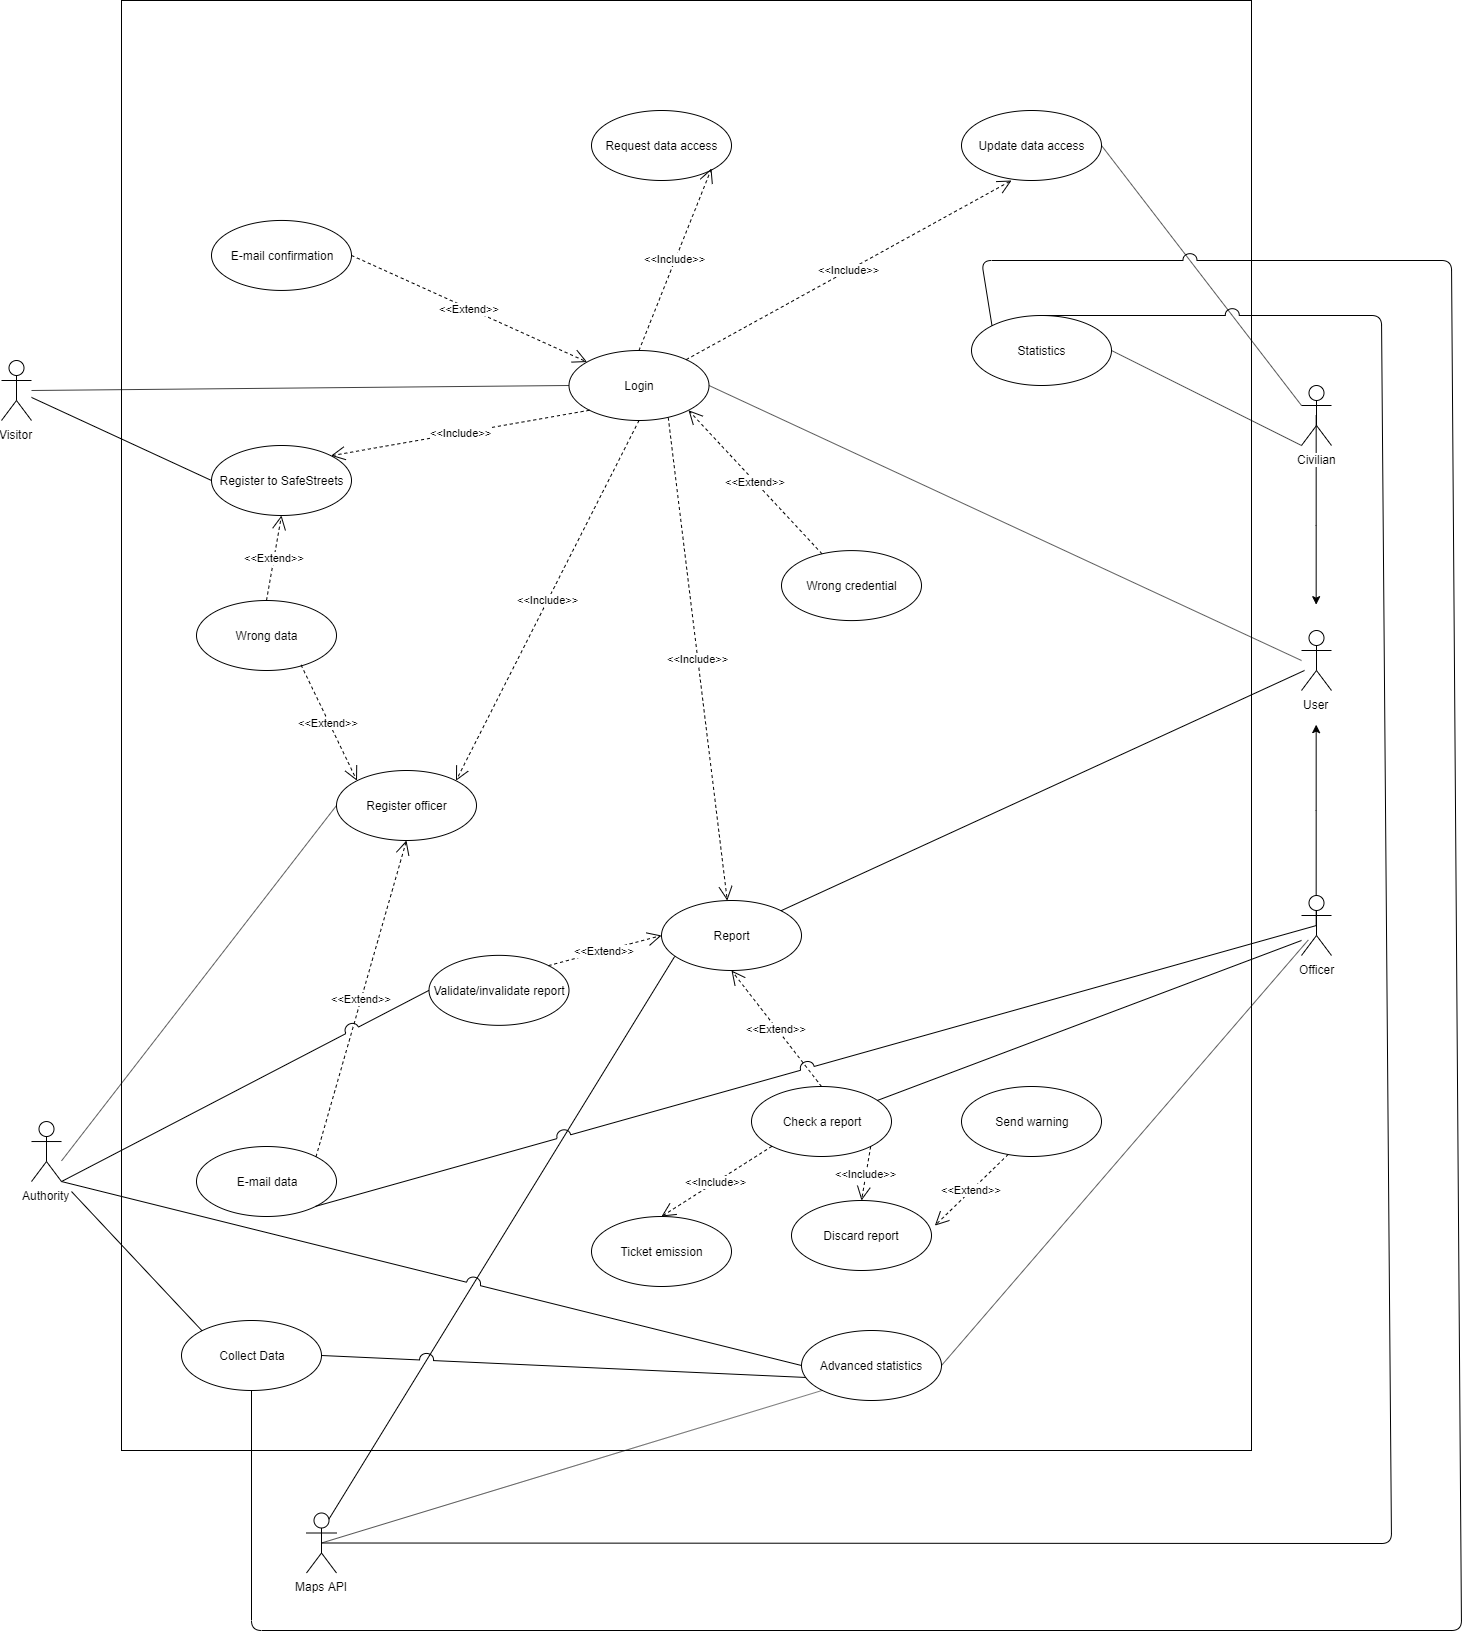
\includegraphics[width=1.2\textwidth,height=.9\textheight]{Images/UseCaseDiagram.png}
	\end{figure}
\subsection{Use cases}
These use case tables describe examples of how the actors may interact with the system to perform the previously listed tasks. An use case about the data collection, processing and representation system has been omitted as the functionality is fully automatized
thus doesn't include any actor.
\subsubsection{Civilian Visitor Registration}
		\begin{center}
			\begin{tabular}{| c | l |}
				\hline
				\textbf{NAME} & Civilian registration \\
				\hline
				\textbf{ACTOR} & Visitor \\
				\hline
				\textbf{GOALS} & [G1] \\
				\hline
				\textbf{ENTRY CONDITIONS} & The Visitor has installed \\
				&	the Application on his/her Mobile device \\ \hline
				\textbf{EVENTS FLOW}  &
				1. Fill all mandatory fields in the Civilian Registration Form\\
				&2. The visitor clicks on "Register" button\\
				&3. The system checks data has not been used already\\
				&4. The system sends an email as confirmation\\
				&5. The system saves Users' data\\
				\hline
				\textbf{EXIT CONDITIONS}  & The Visitor has clicked in the email's link\\ \hline
				\textbf{EXCEPTIONS} &
				1. The email is already registered\\
				&2.  Some mandatory fields are not filled\\
				\hline
			\end{tabular}
		\end{center}

\subsubsection{Civilian Login}
		\begin{center}
			\begin{tabular}{| c | l |}
				\hline
				\textbf{NAME} & Civilian Login \\
				\hline
				\textbf{ACTOR} & Civilian \\
				\hline
				\textbf{GOALS} & [G1] \\
				\hline
				\textbf{ENTRY CONDITIONS} & The civilian is in the Civilian Login page \\ \hline
				\textbf{EVENTS FLOW}  &
				1. The civilian enters his email\\
				&2. The civilian enters the password\\
				&3. The civilian clicks on "Login" button\\
				&4. The system checks the correctness of the credentials\\
				\hline
				\textbf{EXIT CONDITIONS}  & The civilian has successfully logged in \\ \hline
				\textbf{EXCEPTIONS} &
				1. The civilian is not registered\\
				&2. The email is wrong\\
				&3. The password is wrong\\
				&4. Some mandatory fields are not filled\\
				\hline
			\end{tabular}
		\end{center}
\newpage
\subsubsection{Officer Registration}
		\begin{center}
			\begin{tabular}{| c | l |}
				\hline
				\textbf{NAME} & Register to SafeStreets \\
				\hline
				\textbf{ACTOR} & Authority \\
				\hline
				\textbf{GOALS} & [G1] \\
				\hline
				\textbf{ENTRY CONDITIONS} &1.The authority has installed \\
				&	the web application \\
				&2. The authority has a correctly configured server \\ \hline
				\textbf{EVENTS FLOW}  &
				1. Launch the web application\\
				&2. The authority personnel clicks on the \\
				& "Register new officer" button \\
				&3. The authority adds the officer's badge ID and email\\
				&4. The server checks the data has not been used already \\
				&5. The server sends an email with an \\
				& automatically generated password to the officer\\
				&6. The system saves the officer's data\\
				\hline
				\textbf{EXIT CONDITIONS}  & The email has successfully been sent to the officer\\ \hline
				\textbf{EXCEPTIONS} &
				1. The badge is already registered\\
				&2. The email is already registered\\
				&3. Some mandatory fields are not filled\\
				\hline
			\end{tabular}
		\end{center}

\subsubsection{Officer Login}
		\begin{center}
			\begin{tabular}{| c | l |}
				\hline
				\textbf{NAME} & Officer Login \\
				\hline
				\textbf{ACTOR} & Officer \\
				\hline
				\textbf{GOALS} & [G1] , [G.5.2] \\
				\hline
				\textbf{ENTRY CONDITIONS} &1. The officer has downloaded the mobile application \\
				&2.The officer has seen the password in his email\\
				&3.The officer is in the Officer Login page \\ \hline
				\textbf{EVENTS FLOW}  &
				1. The officer enters his badge ID\\
				&2. The officer enters his password\\
				&3. The officer clicks on "Login" button\\
				&4. The system checks the correctness of the credentials\\
				&5. The officer chooses a 5 digit pin to emit tickets \\ \hline
				\textbf{EXIT CONDITIONS}  & The officer has successfully logged in \\ \hline
				\textbf{EXCEPTIONS} &
				1. The officer is not registered\\
				&2. The badge ID is wrong\\
				&3. The password is wrong\\
				&4. Some mandatory fields are not filled\\
				\hline
			\end{tabular}
		\end{center}

\subsubsection{Violation reporting}
		\begin{center}
			\begin{tabular}{| c | l |}
				\hline
				\textbf{NAME} & Violation reporting \\
				\hline
				\textbf{ACTOR} & User \\
				\hline
				\textbf{GOALS} & [G2] ,[G4], [G.5.1] \\
				\hline
				\textbf{ENTRY CONDITIONS} &1.The user is logged in \\
				&2. The user has allowed the app \\
				&to use the camera and GPS \\ \hline
				\textbf{EVENTS FLOW}  &
				1. The user clicks on "Report"\\
				&2. The user chooses a violation from the \\
				& dropdown menu \\
				&3. The user takes a pic of the vehicle and \\
				& the violation being committed \\ \hline
				&4. The user frames the license plate\\
				&5. The system computes the plate number \\
				&6. The system checks if the report is a duplicate\\
				&7. The system adds date and timestamp \\
				& and sends the report to the authority \\ 
				\hline
				\textbf{EXIT CONDITIONS}  & The report has successfully been sent \\ \hline
				\textbf{EXCEPTIONS} &
				1. The plate can't be recognised \\
				&2. The report is a duplicate\\
				&3. GPS is turned off\\
				&4. Camera can't be used for any reason\\
				\hline
			\end{tabular}
		\end{center}

\subsubsection{Ticket confirmation}
		\begin{center}
			\begin{tabular}{| c | l |}
				\hline
				\textbf{NAME} & Ticket confirmation \\
				\hline
				\textbf{ACTOR} & Officer \\
				\hline
				\textbf{GOALS} & [G2] ,[G4], [G.5.3] \\
				\hline
				\textbf{ENTRY CONDITIONS} &1. The Officer is logged in \\
				&2. The officer is near a reported violation \\
				&3. The plate number matches the one \\
				& contained in the report\\ \hline
				\textbf{EVENTS FLOW}  &
				1. The officer inserts his pin \\
				&2. The officer clicks on the "Send" button\\	
				&3. The system checks the pin's correctness \\
				&4. The system sends a notice to the authority \\
				&5. The system deletes the report from the map \\ 
				\hline
				\textbf{EXIT CONDITIONS}  & The confirmation has successfully been sent \\ \hline
				\textbf{EXCEPTIONS} &
			 The pin is wrong \\
				\hline
			\end{tabular}
		\end{center}

\subsubsection{Report validation}
		\begin{center}
			\begin{tabular}{| c | l |}
				\hline
				\textbf{NAME} & Report validation \\
				\hline
				\textbf{ACTOR} & Authority \\
				\hline
				\textbf{GOALS} & [G2] ,[G3], [G.5.1] \\
				\hline
				\textbf{ENTRY CONDITIONS} &1. The Authority is in the main menu \\
				&2. The authority received a violation report \\ \hline
				\textbf{EVENTS FLOW}  &
				1. The authority checks the photo correctness\\
				&2. The authority clicks "Validate" \\
				&3. The system adds the report to  \\
				& the data warehouse \\
				&4. The system adds the report to the map \\ 
				&5. The server sends notifications to \\
				& active officers. \\
				\hline
				\textbf{EXIT CONDITIONS}  & The report has been validated \\ \hline
				\textbf{EXCEPTIONS} & None \\
				\hline
			\end{tabular}
		\end{center}

\subsubsection{Report invalidation with warning}
		\begin{center}
			\begin{tabular}{| c | l |}
				\hline
				\textbf{NAME} & Report invalidation \\
				\hline
				\textbf{ACTOR} & Authority \\
				\hline
				\textbf{GOALS} & [G2] ,[G3], [G.5.1] \\
				\hline
				\textbf{ENTRY CONDITIONS} &1. The Authority is in the main menu \\
				&2. The authority received a violation report \\ \hline
				\textbf{EVENTS FLOW}  &
				1. The authority checks the photo correctness\\
				&2. The authority clicks "Validate " \\
				&3. The authority clicks on "Warn"  \\
				&4. The server sends a ban request to \\
				& the SafeStreets server \\
				\hline
				\textbf{EXIT CONDITIONS}  & The report has been invalidated \\ \hline
				\textbf{EXCEPTIONS} & None \\
				\hline
			\end{tabular}
		\end{center}

\subsection{Sequence diagrams}
\subsubsection{Visitor to Civilian Registration}
			\begin{figure}[H]
				\centering
				\includegraphics[width=.9\textwidth,height=.9\textheight,keepaspectratio]{Images/registration_sequence}
				\label{fig:registration_sequence}
			\end{figure}
		\subsubsection{Officer Registration}
Also includes the first login in which the 5 digit pin is compiled, to complete the registration sequence.
			\begin{figure}[H]
				\centering
				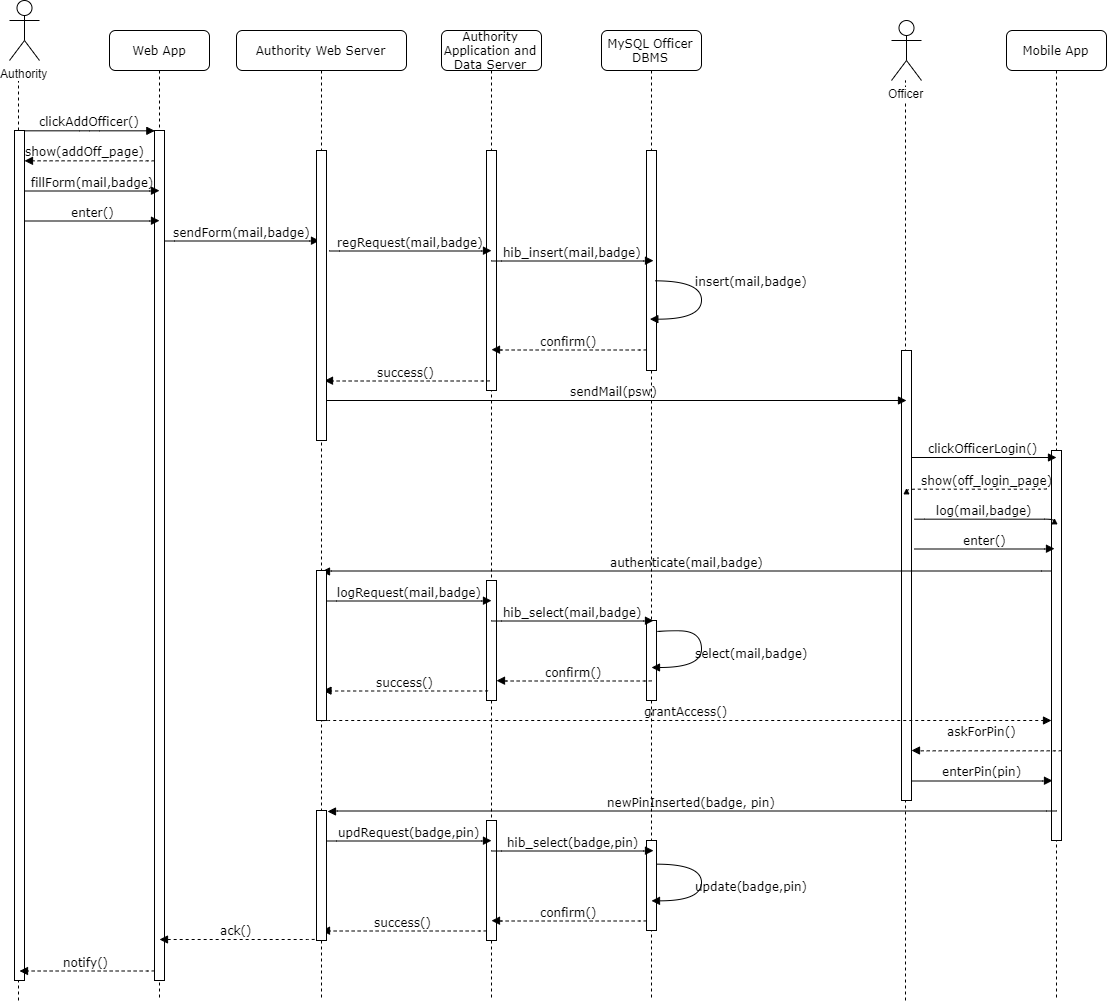
\includegraphics[width=.9\textwidth,height=.9\textheight,keepaspectratio]{Images/Off_registration}
				\label{fig:login_sequence}
			\end{figure}
		\subsubsection{Correct violation report}
			\begin{figure}[H]
				\centering
				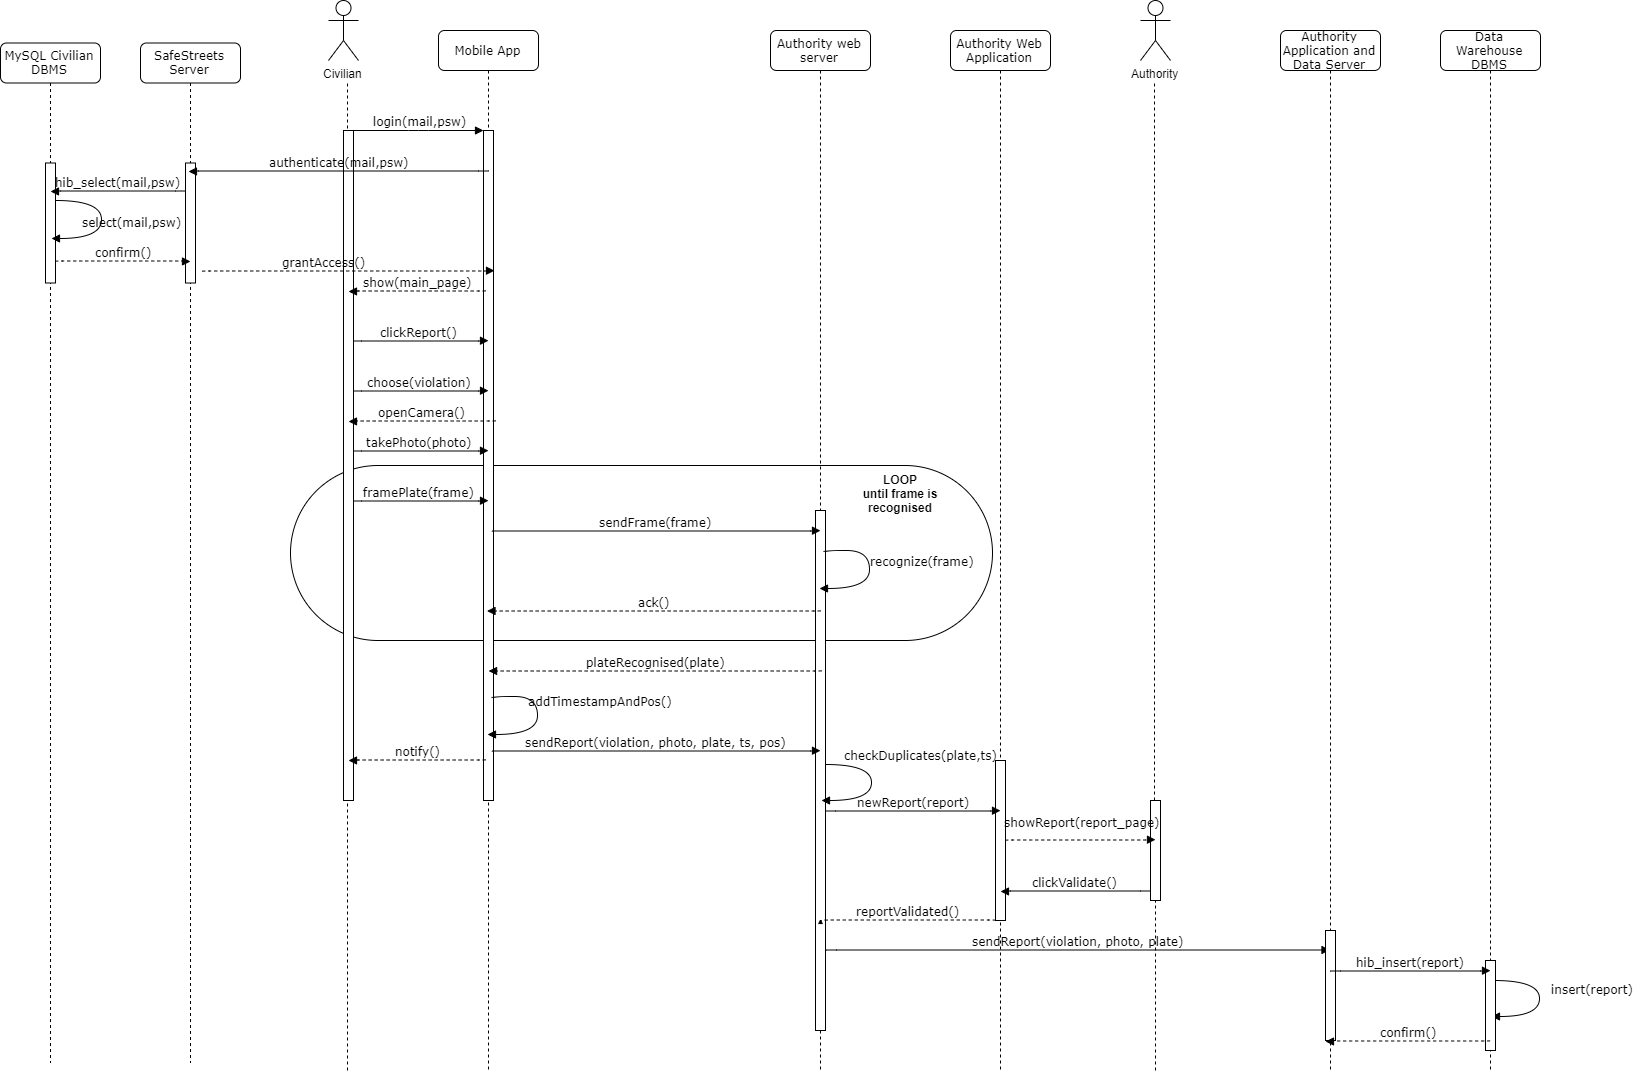
\includegraphics[width=1.2\textwidth,height=.9\textheight]{Images/Civilian_report}
				\label{fig:request_subscription_sequence}
			\end{figure}
		\subsubsection{Invalid violation with subsequent banning}
			\begin{figure}[H]
				\centering
				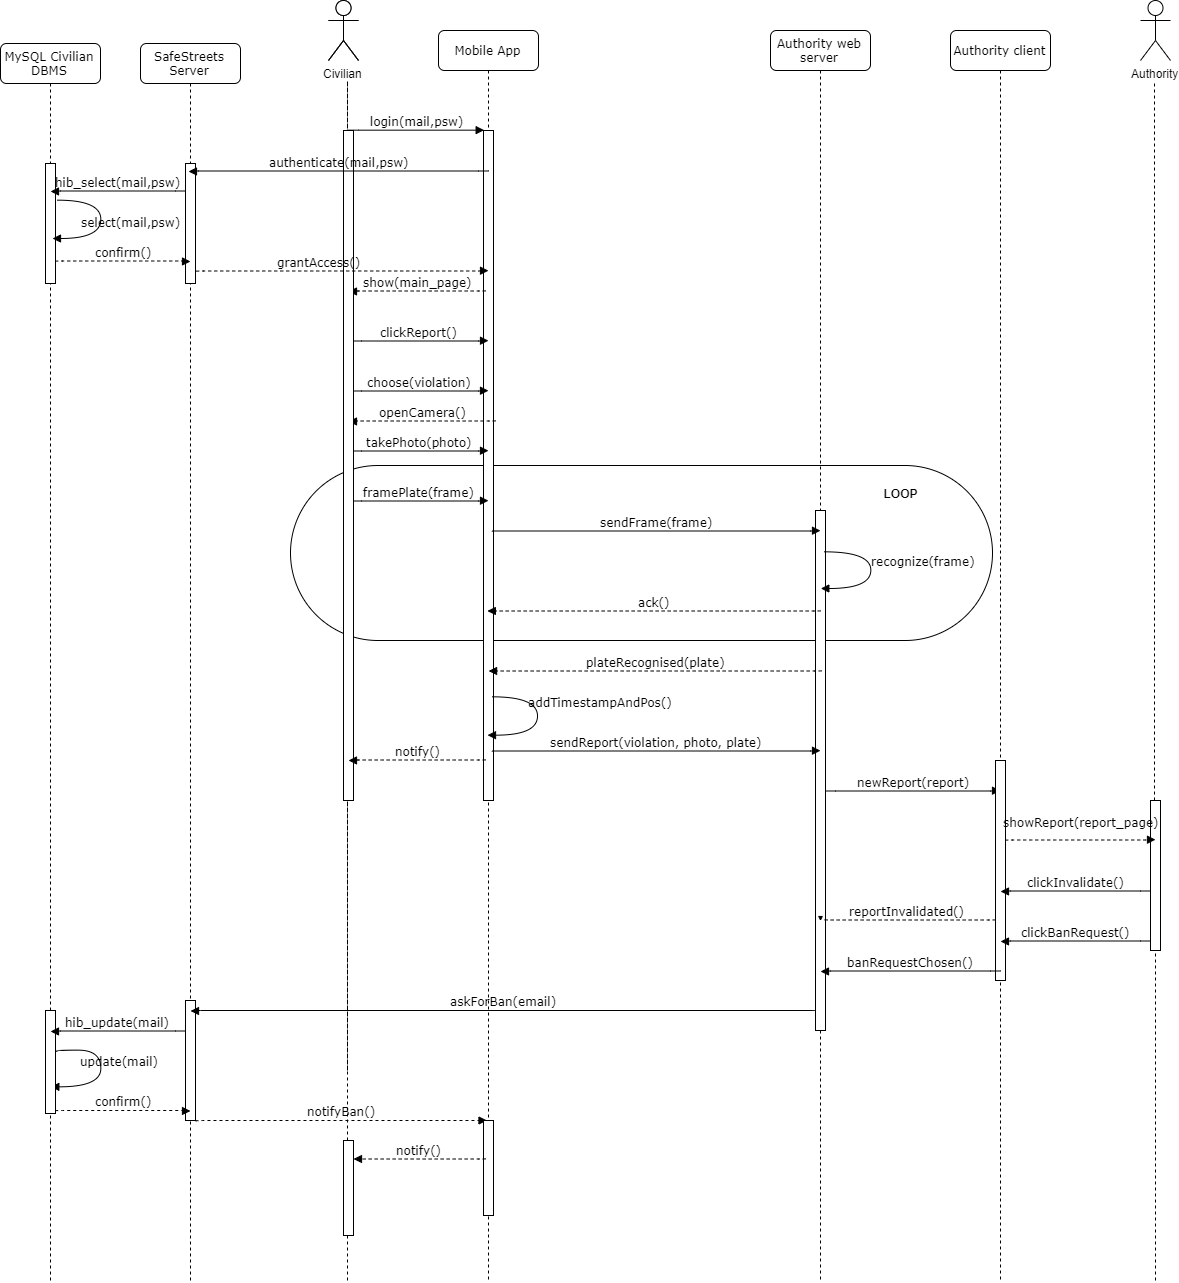
\includegraphics[width=.9\textwidth,height=.9\textheight,keepaspectratio]{Images/invalidation_banning}
				\label{fig:ass_request_sequence}
			\end{figure}
		\subsubsection{Automated Ticket}
			\begin{figure}[H]
				\centering
				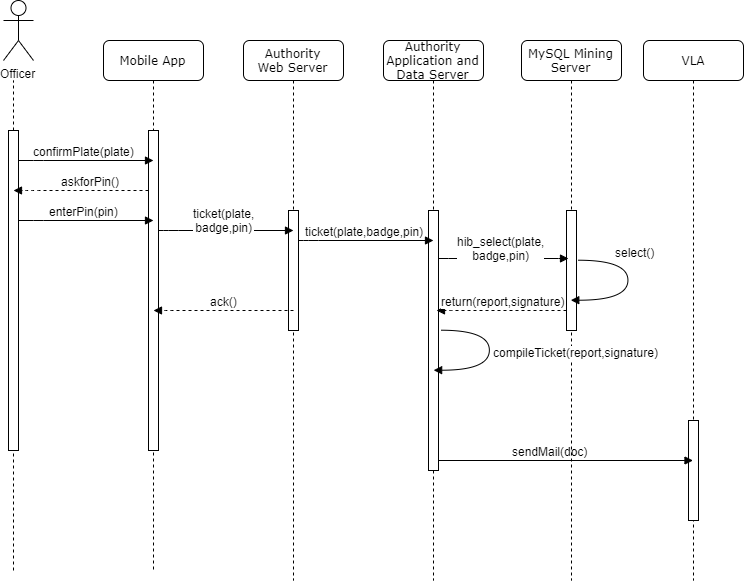
\includegraphics[width=.9\textwidth,height=.9\textheight,keepaspectratio]{Images/automated_ticket}
				\label{fig:automated_request_sequence}
			\end{figure}
\newpage
		\subsubsection{Update sending}
			\begin{figure}[H]
				\centering
				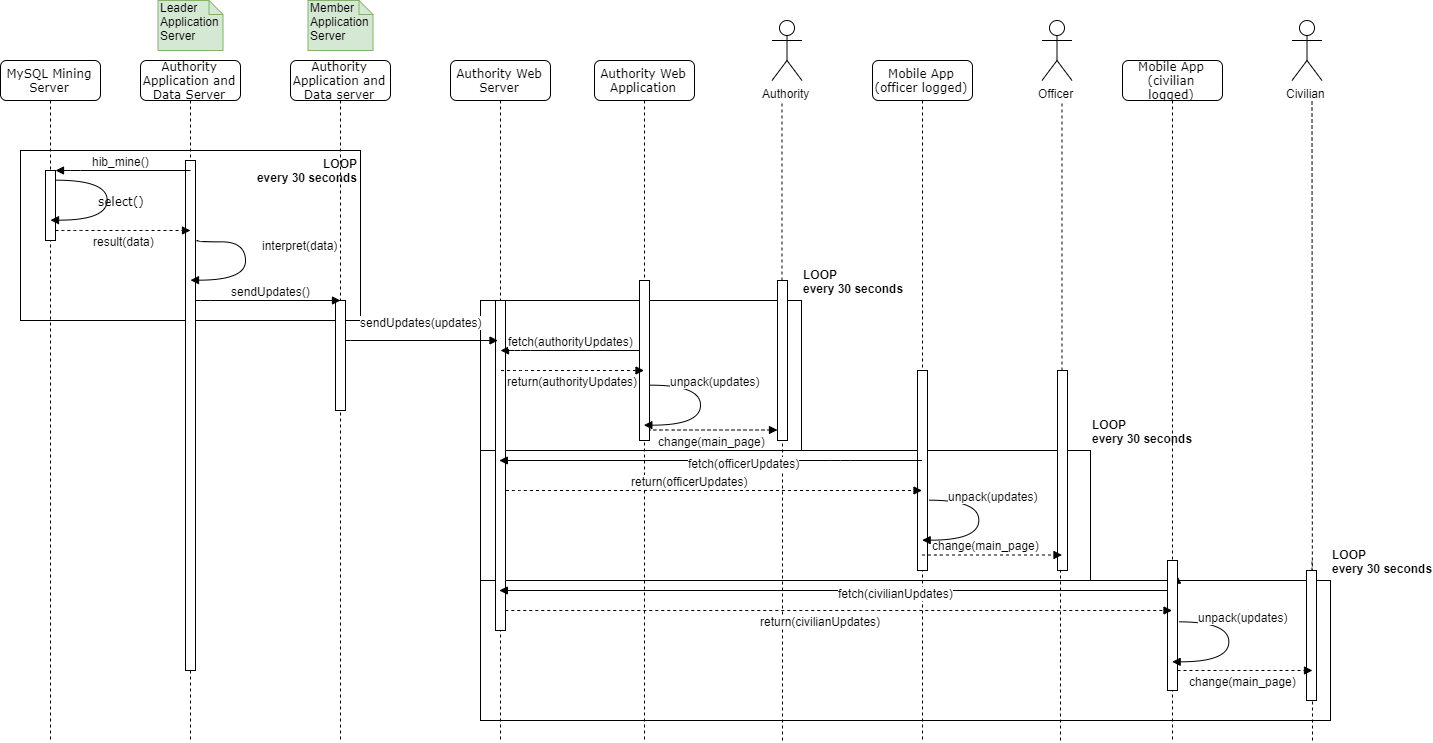
\includegraphics[width=.9\textwidth,height=.9\textheight,keepaspectratio]{Images/update_sending}
				\label{fig:sampling_request_sequence}
			\end{figure}

\subsection{Performance	Requirements}
In general, the software should be an helpful tool for authorities and thus its efficient use strongly depends on their ability to use it readily.By assuming reliable links and decent performance of network protocol communications, mailing services etc. the throughput of the system mostly depends on the personnel operating the web application and the officer (as reports cannot be converted into fines without their validation). In the presence of multiple reports and multiple authorities processing them, like what would possibly happen in big cities, the system has nonetheless to guarantee the time bounds specified in the requirements for the sending of new processed data, and especially swiftly notify new reports. Reports must be guaranteed to expire after a customizable time limit has expired, to make sure that no effort is wasted by officers in checking old ones. 
\subsection{Design	Constraints}
\subsubsection{Hardware Limitations}
		\begin{itemize}
			\item \texttt{Mobile App}: 
				\begin{itemize}
					\item Smartphones: Android or iOS, Internet Connection, GPS.
				\end{itemize}
			\item \texttt{Web App}: modern web browser (e.g. Google Chrome / Safari) able to support a Rich Internet Application, Internet connection.
		\end{itemize}
\subsubsection{Standards	compliance}
The system uses the International System of Units as it system of measurements and the sensitive data will be treated according to the General Data Protection Regulation rules.
\subsection{Software	 System	 Attributes} 
\subsubsection{Reliability}
The system should always be able to process reports and store them in the data warehouse, but according to G1 the priority is assisting law enforcers and not substituting the existing procedures, thus transient and occasional deviations can be accepted.  Reports can be processed by multiple authorities' servers if the previous one fail (e.g. every police barrack has a server), so replication will be used to guarantee both availability and reliability.
\subsubsection{Availability}
The system must fullfil all the registration, login requests and reports whenever needed, only a small percentage of requests missed (around 0.1\%) can be tolerated. 
\subsubsection{Security}
Officers information is stored in the authorities' data server and not in SafeStreets', which only hosts civilian accounts. Through the badge-password authentication and the fact that only authorities can add officers, it will be impossible for civilians to log in as officers, and even if in some way someone who is not an officer is able to access to an officer account, he will not be able to do any substantial harm because of the pin required to sign tickets. A timeout will also automatically log the officer out. Authorities can see in real time every active officer through their client, so they also may be able to notice inconsistencies. Invalid reports will be discarded at the authority's client, and users will not be allowed to upload images to make sure every report photo is taken in real time and not manipulated. Similarly, the license plate will be scanned through an accurate supervised learning algorith run on the client so that it can not be input by a fraudolent user: officers will have the duty to later check the correctness of the plate number when signing the ticket.
The system will also guarantee to not spread any kind of data to third parties to accomplish goal G7.
\subsubsection{Maintainability}
Best practices and design patterns of Object Oriented Programming along with documentation upkeep will be thoroughly followed to make sure the application is easily customizable and modifiable by SafeStreets' developers.
\subsubsection{Scalability}
The architecture must be simply scalable as the number of users grows over time. Except civilian account management, which is handled by SafeStreets' server and should not require too much complexity, functions are mostly provided by the authorities' servers which grow in number with the population of the considered city (e.g. the bigger the city the more numerous the barracks, and therefore the number of servers), thus the architecture will be scalable by design. In any case, the number of reports per day should never exceed a few thousands even in heavily populated cities.
\newpage
\section{FORMAL ANALYSIS USING ALLOY}
\subsection{Purpose of the analysis}
In this section we provide a formalization of some constraints on how the entities of the system will interact, and the formalization of some non-functional requirements:
\begin{itemize}
 \item how reports are accepted or rejected due to duplicates not being allowed and the authority manually discarding them;
 \item how map updates are controlled by the reports and how the reports they contain expires;
 \item how bans restrict the actions of civilians;
 \item how the report checking done by officers happens and how that controls ticket emission;
 \item various constraints on users' data.
\end{itemize}
\newpage
\subsection{Analysis}

\subsubsection{Signatures}
\begin{figure}[H]
				\centering
				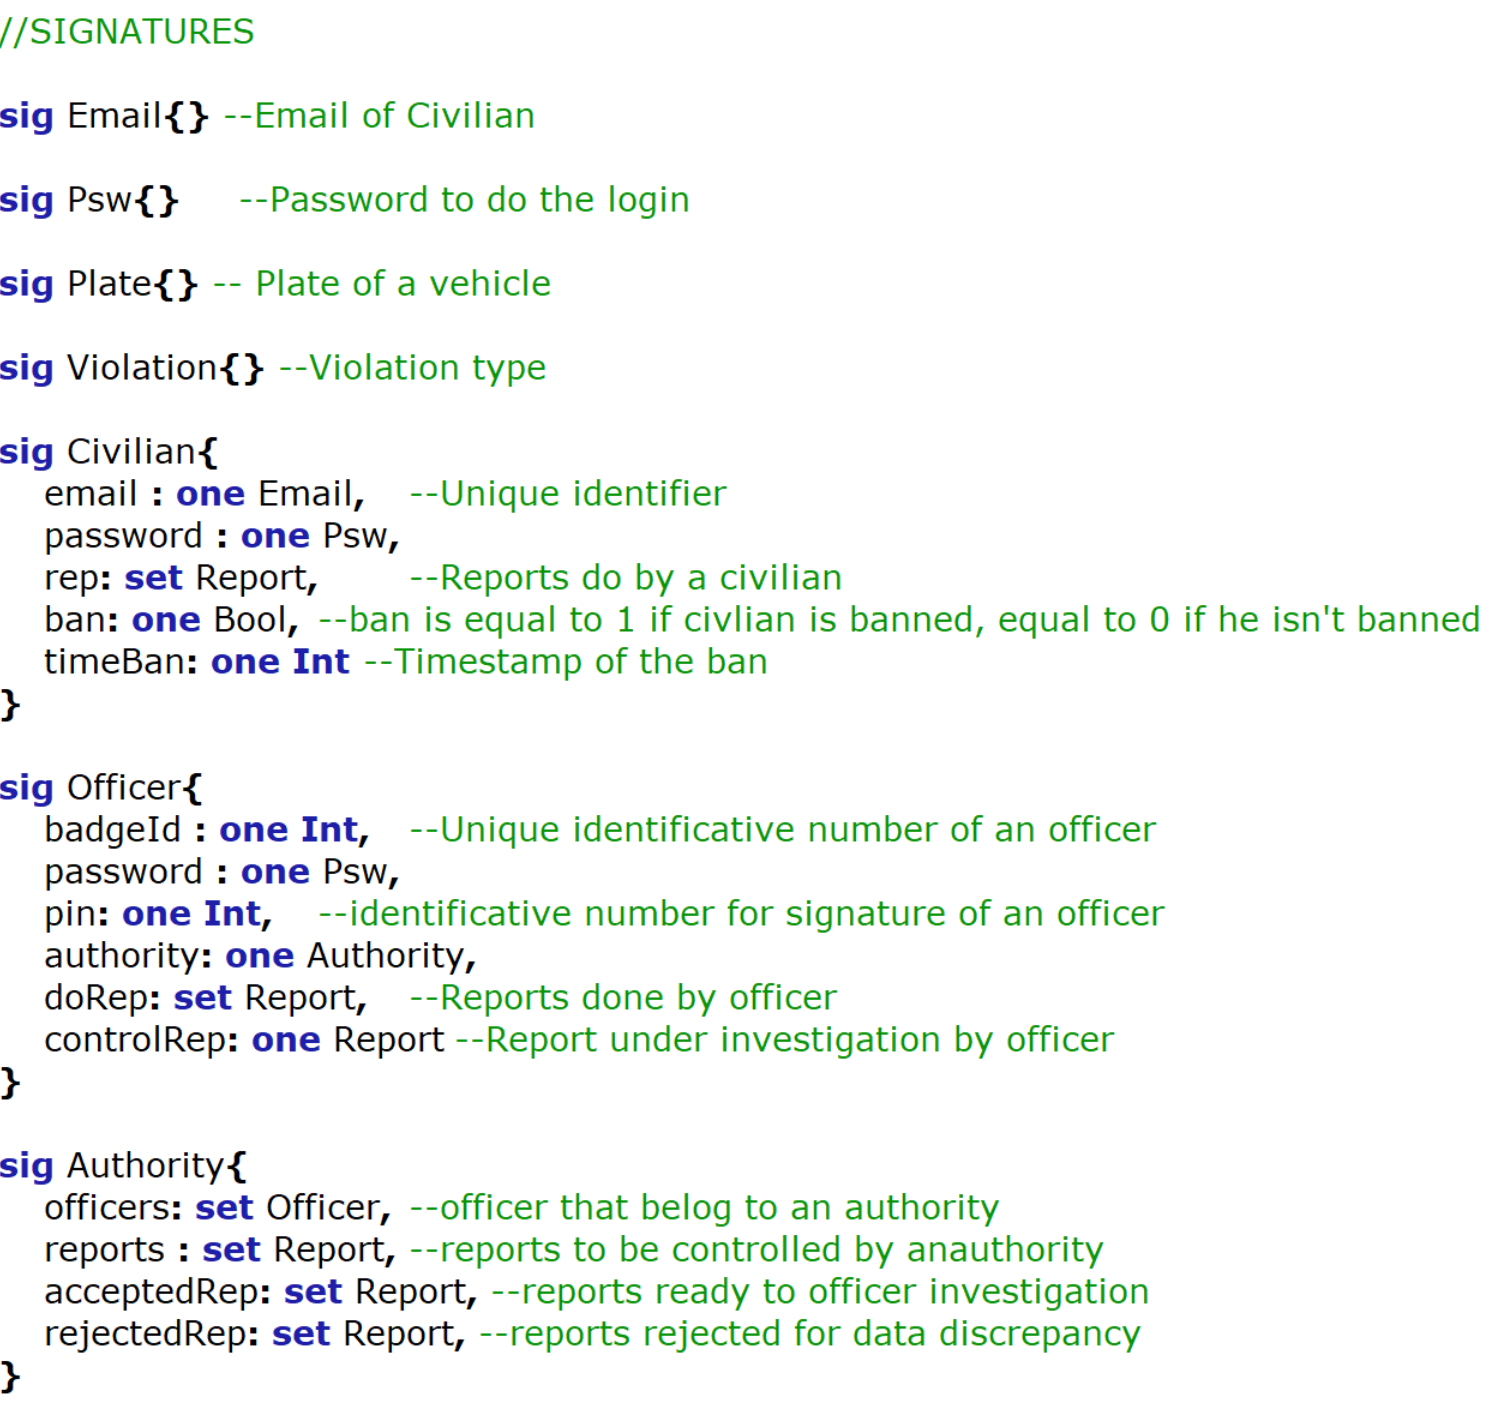
\includegraphics[width=.75\paperwidth,height=.75\paperheight, keepaspectratio]{Images/Alloy/sig1}
\end{figure}
\begin{figure}[H]
				\centering
				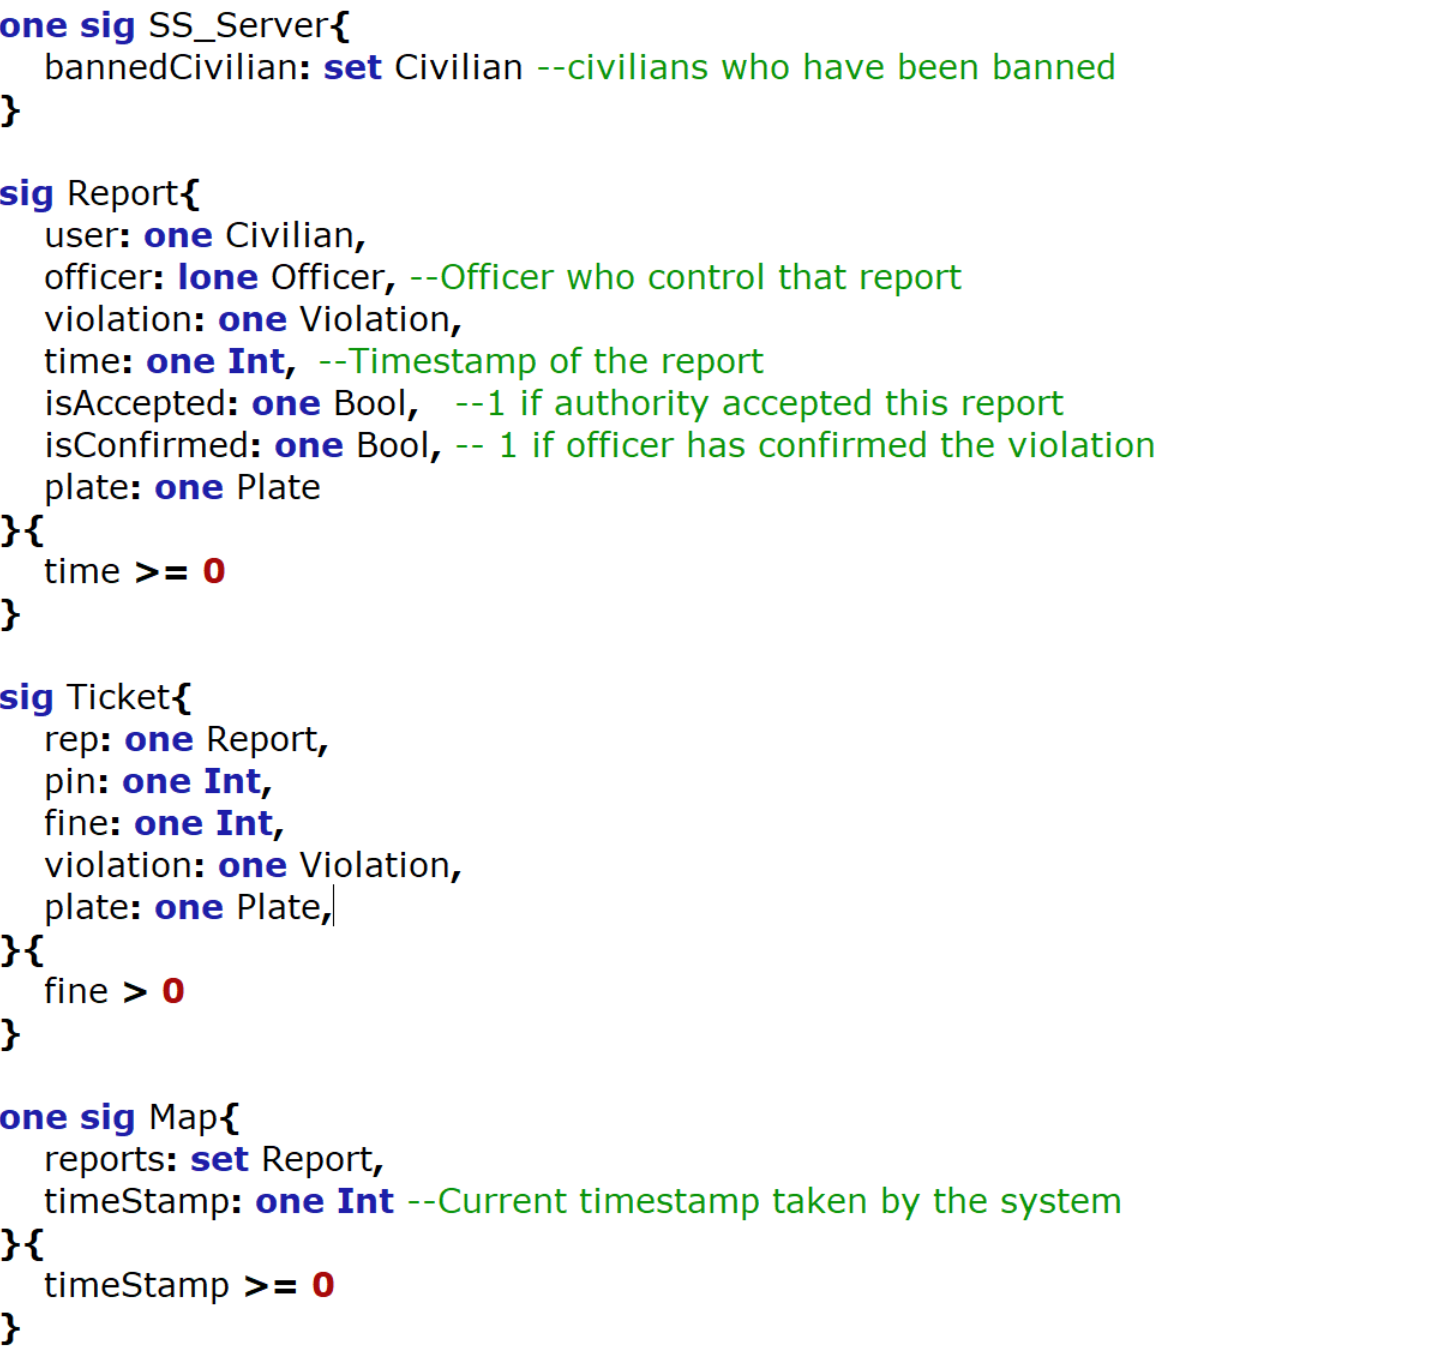
\includegraphics[width=.7\paperwidth,height=.7\paperheight, keepaspectratio]{Images/Alloy/sig2}
\end{figure}

\subsubsection{Facts}

\begin{figure}[H]
				\centering
				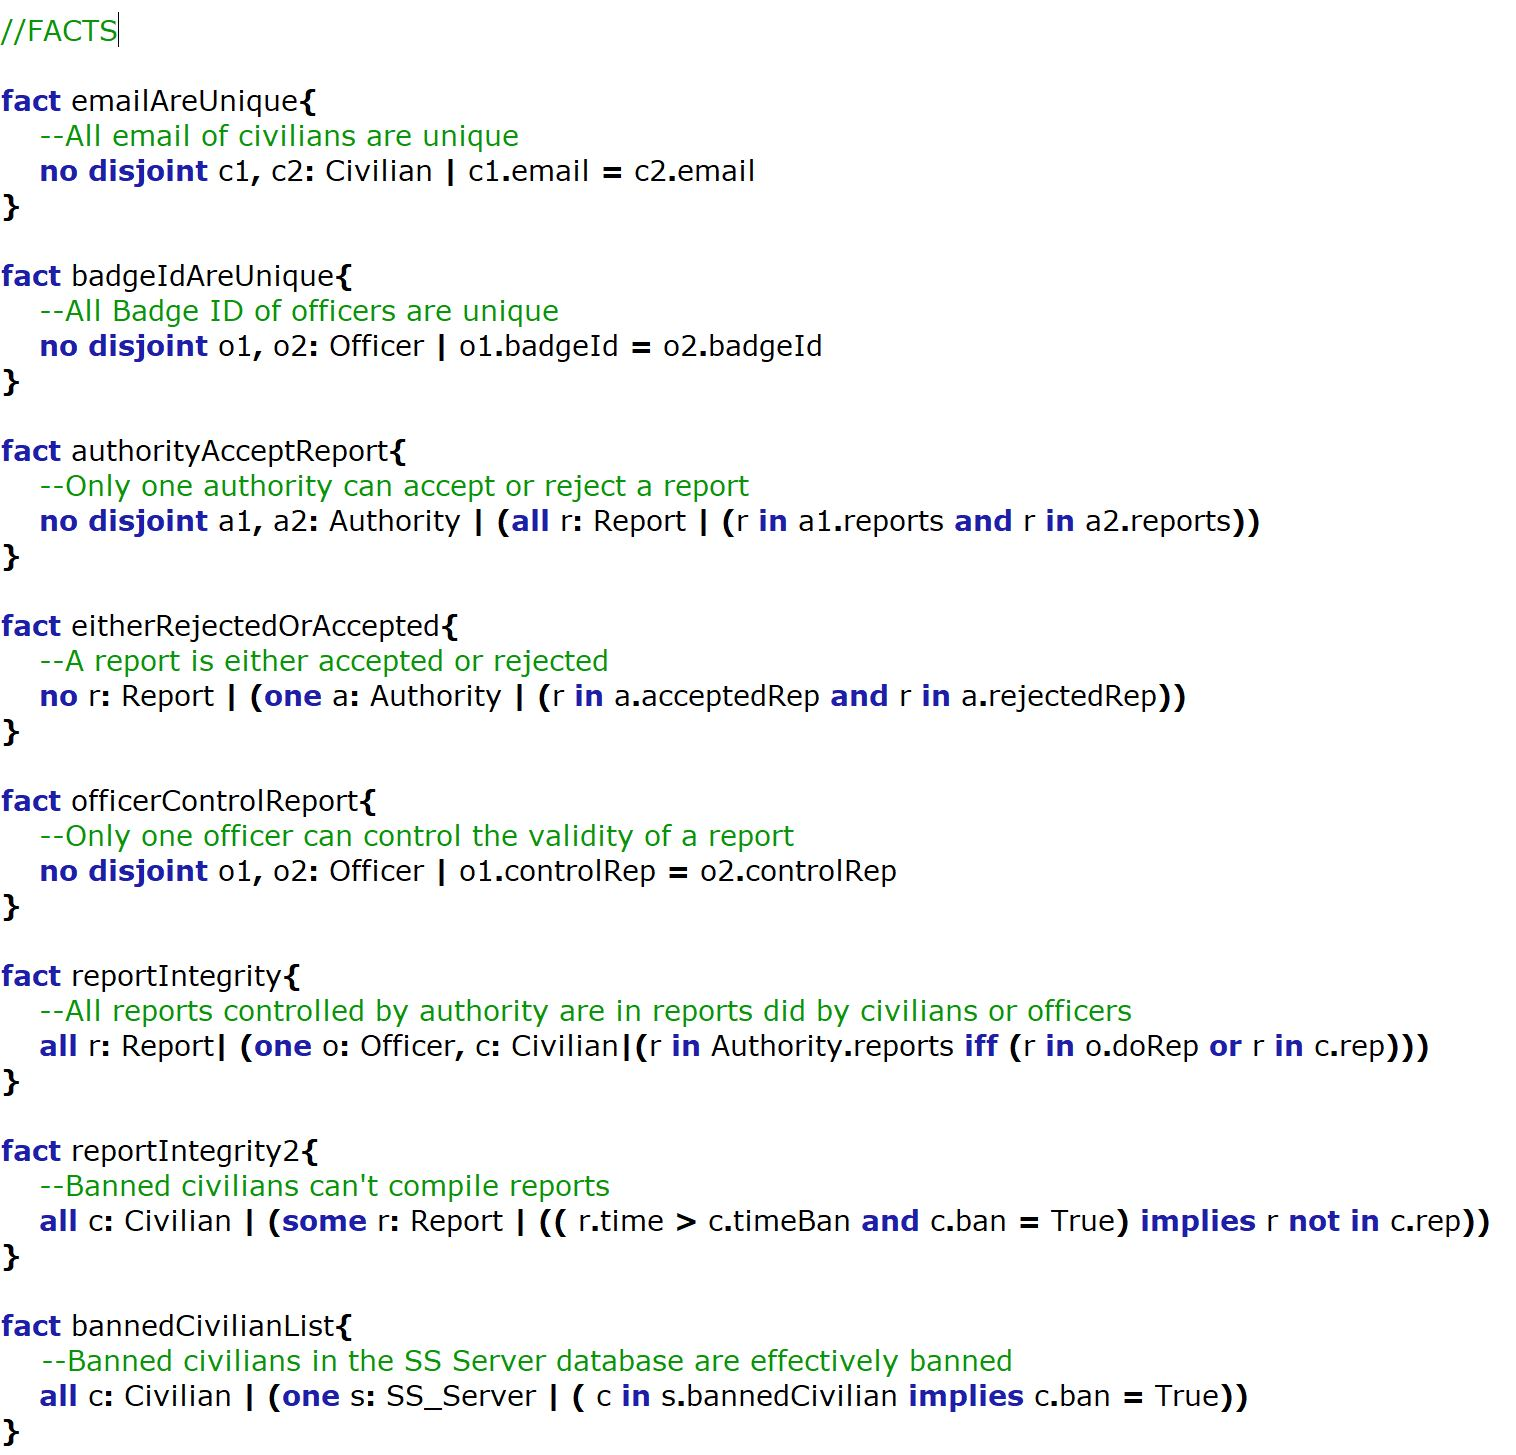
\includegraphics[width=.75\paperwidth,height=.75\paperheight, keepaspectratio]{Images/Alloy/facts1}
\end{figure}
\begin{figure}[H]
				\centering
				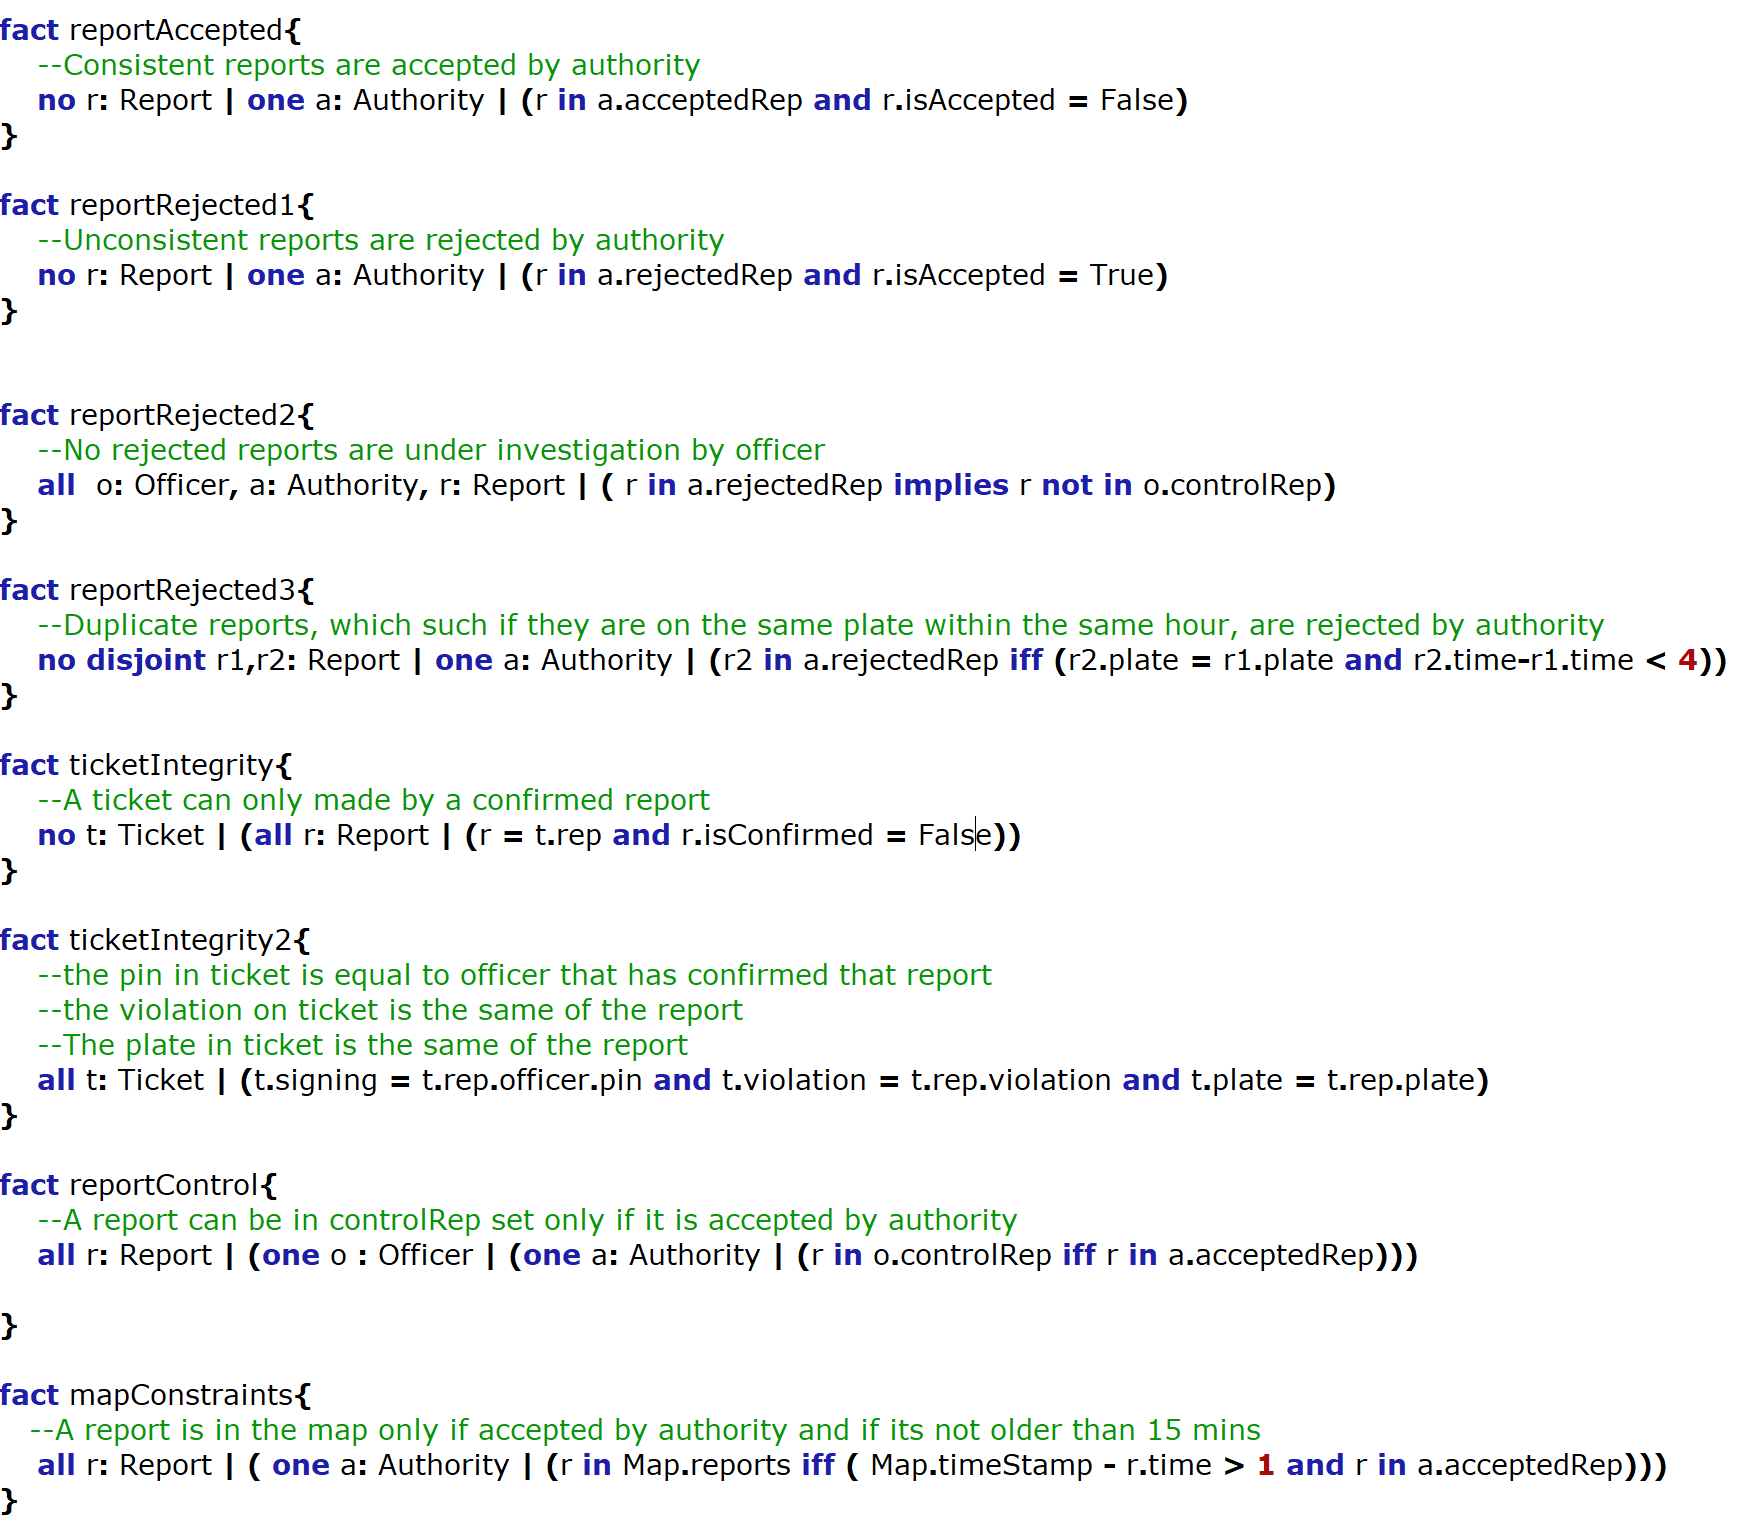
\includegraphics[width=.75\paperwidth,height=.75\paperheight, keepaspectratio]{Images/Alloy/facts2}
\end{figure}

\subsubsection{Assertions}

\begin{figure}[H]
				\centering
				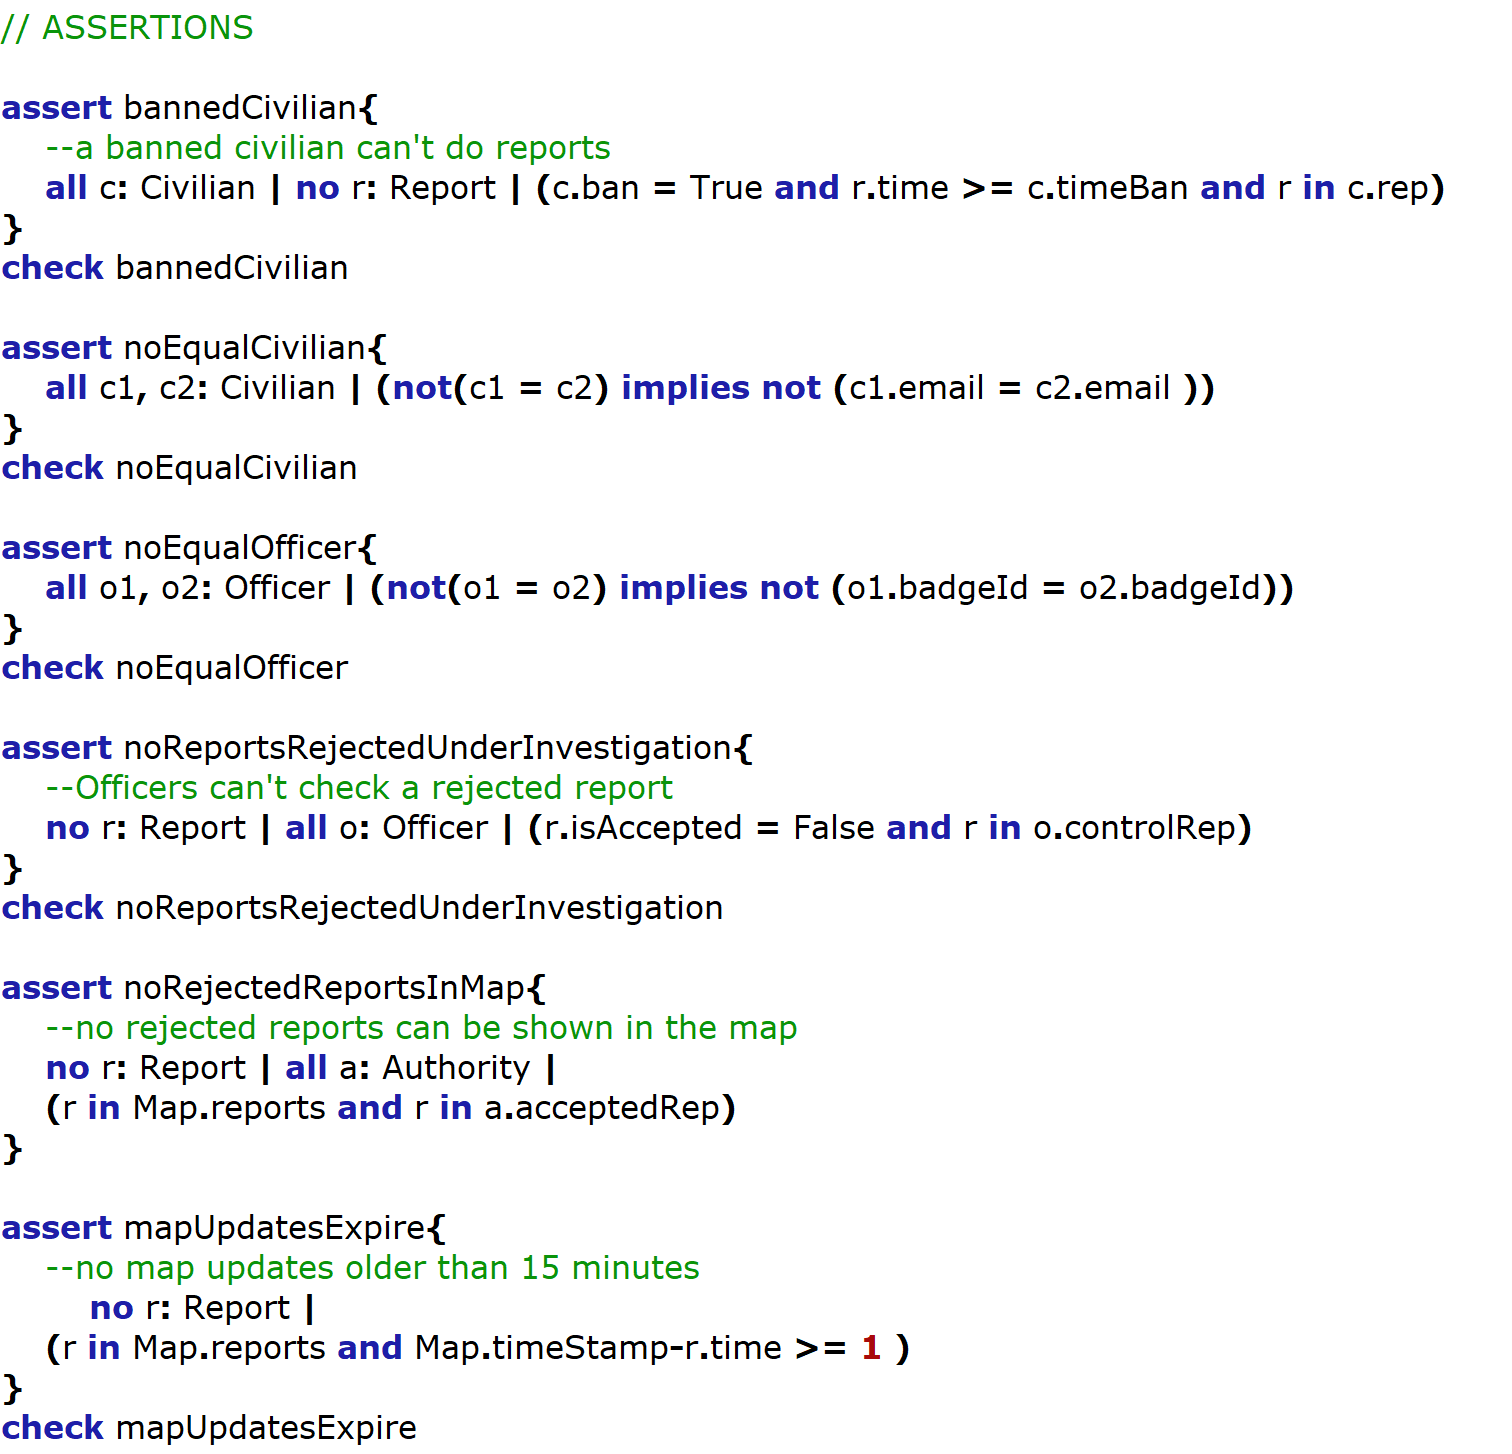
\includegraphics[width=.75\paperwidth,height=.75\paperheight, keepaspectratio]{Images/Alloy/asserts}
\end{figure}

\subsubsection{Results}
\begin{figure}[H]
				\centering
				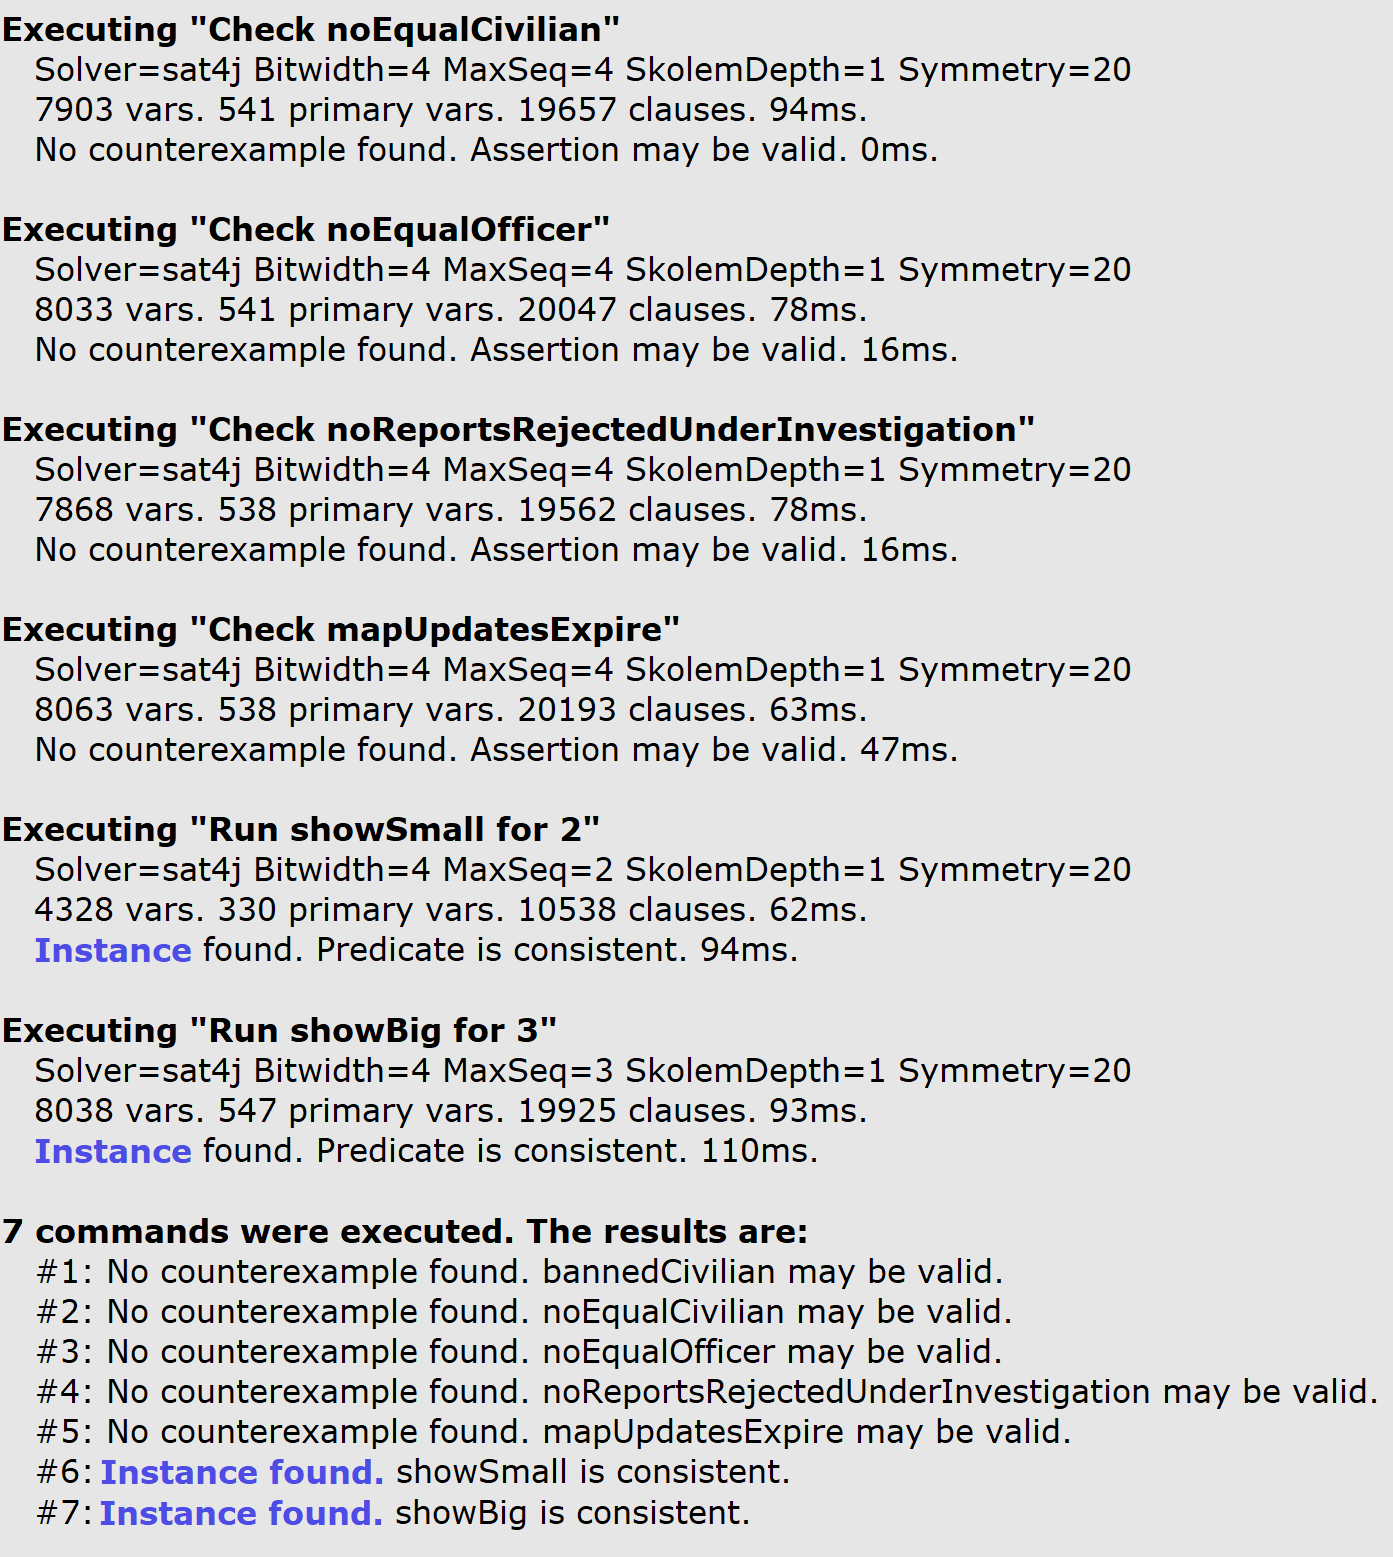
\includegraphics[width=.6\paperwidth,height=.6\paperheight, keepaspectratio]{Images/Alloy/results}
\end{figure}
\subsubsection{Metamodel}
\begin{figure}[H]
				\centering
				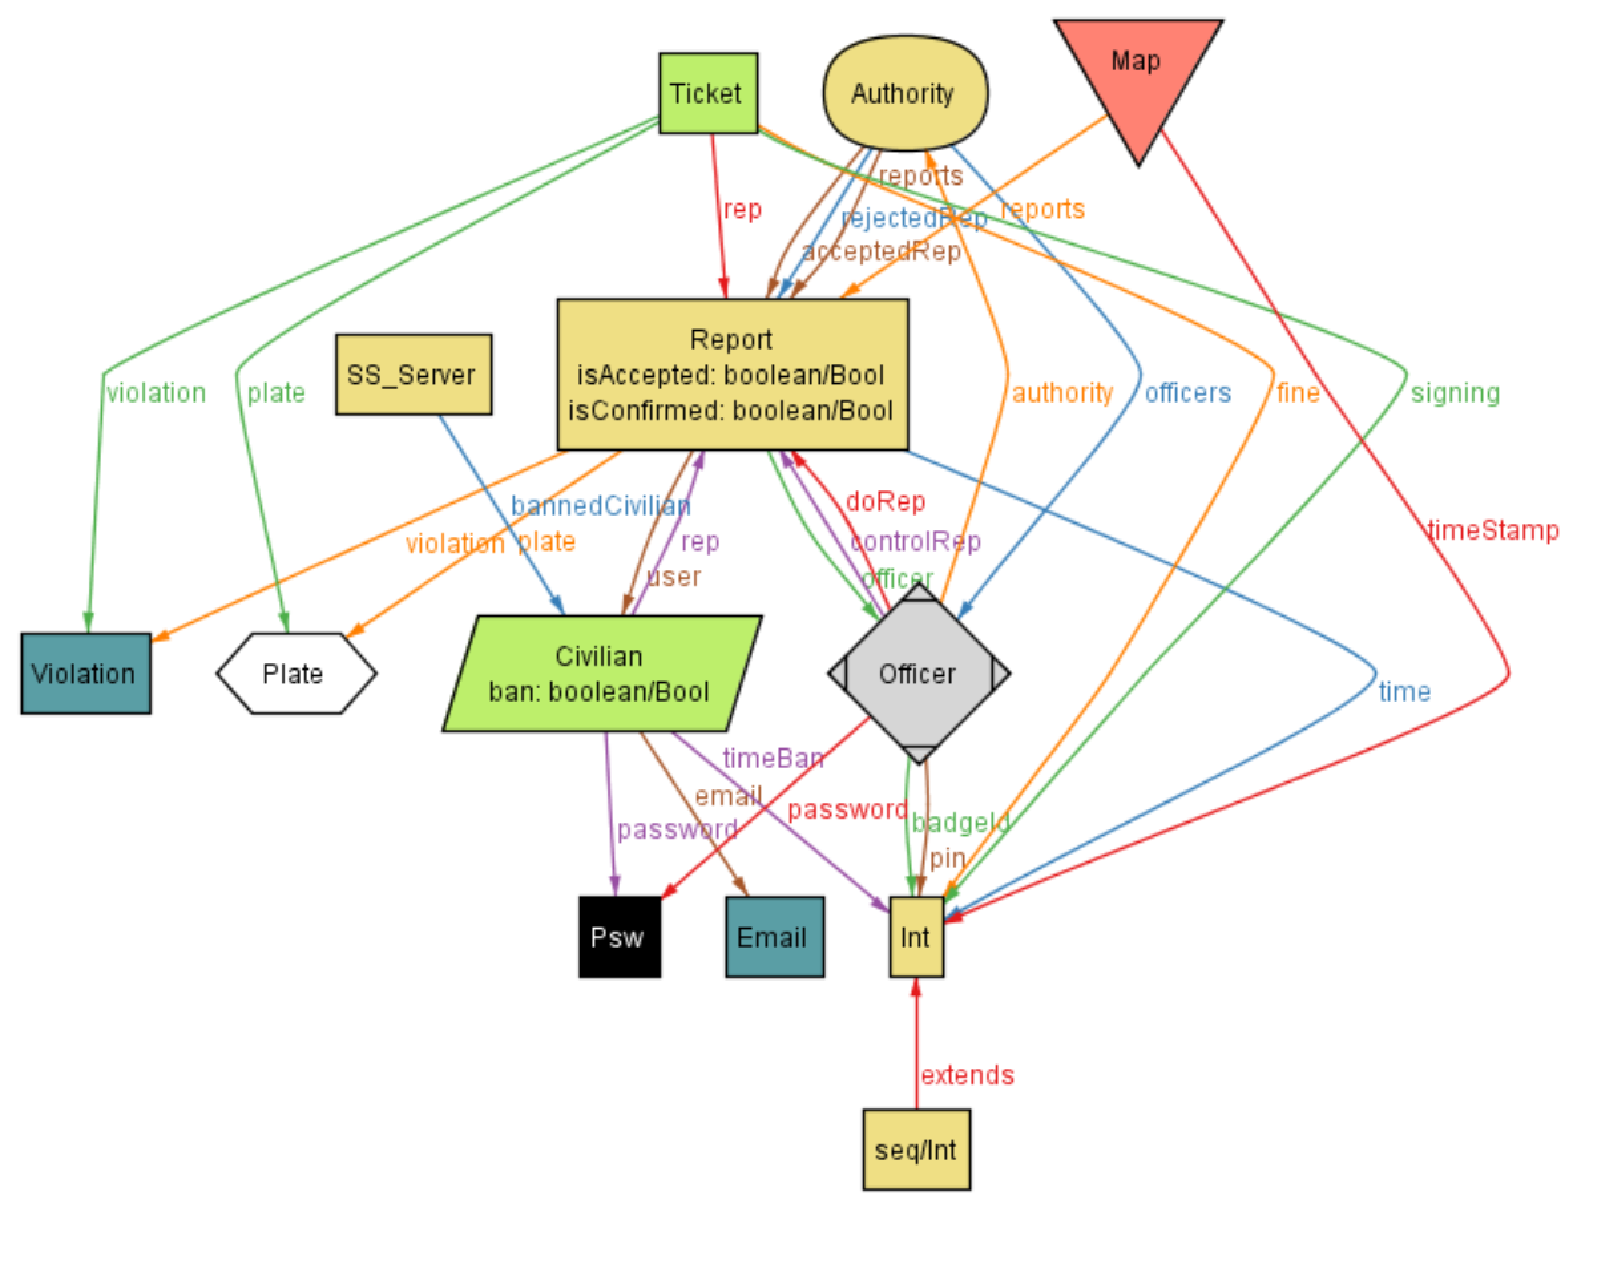
\includegraphics[]{Images/Alloy/metamodel}
\end{figure}
\subsubsection{Generated Worlds}
\begin{figure}[H]
				\centering
				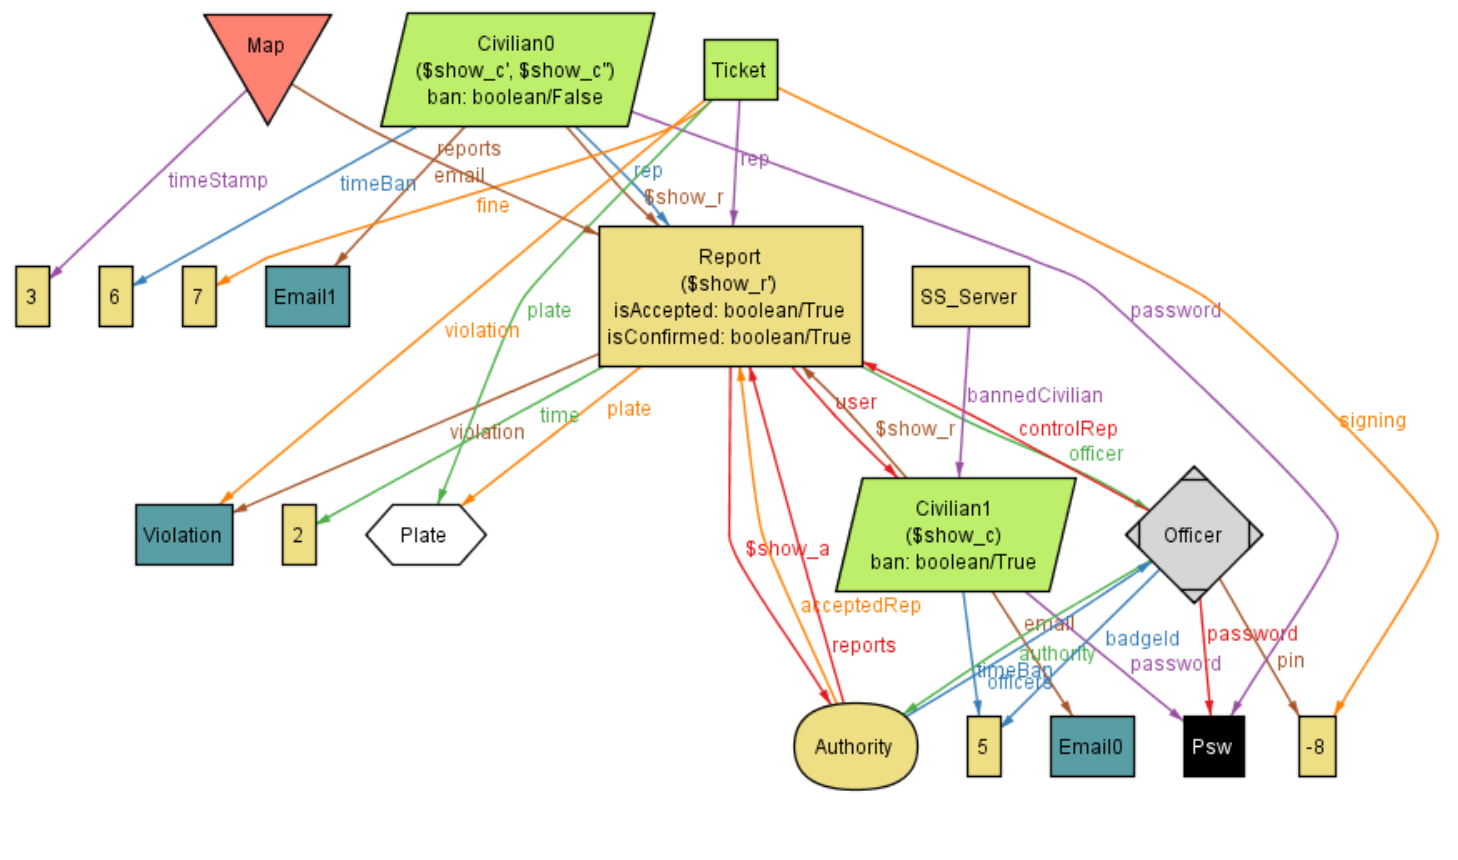
\includegraphics[]{Images/Alloy/world}
\end{figure}
This is the world generated by the predicate \texttt{show}, which evolves around an accepted report, showing the bindings with its map update and the various actors: the report is generated by a civilian and is being controlled by an officer.
We also included a ticket and a banned civilian to better visualize the various restriction to which he is subject.

\newpage
\section{EFFORT	SPENT}
\begin{itemize}
\item {Davide Cocco}
 \begin{center}
			\begin{tabular}{| c | l | c |}
				\hline
				\textbf{Day} & \textbf{Subject} & \textbf{Hours} \\ \hline
				15/10/2019 & Purpose, Scope, Goals, Product functions,&\\
				&User charateristics & 2.5 \\ \hline
				18/10/2019 & Domain assumpions, Scenarios, Software attributes,&\\
				& Use cases, Functional requirements and updates  & 6\\ \hline
				20/10/2019 & Requirements  & 2\\	\hline
				21/10/2019 & Sequence Diagrams  & 2\\ \hline
				20/10/2019 & State Diagrams  & 2\\ \hline
				24/10/2019 & Class Diagram  & 2\\ \hline
				29/10/2019 & Document revision and filling minor sections & 1\\ \hline
				9/11/2019 & Alloy & 5\\ \hline
				Total & & 22.5 \\ \hline
			\end{tabular}
		\end{center}
\item {Marco Gasperini}
\begin{center}
			\begin{tabular}{| c | l | c |}
				\hline
				\textbf{Day} & \textbf{Subject} & \textbf{Hours} \\ \hline
				15/10/2019 & Purpose, Scope, Goals, Product functions,&\\
				&User charateristics & 2.5 \\ \hline
				18/10/2019 & Domain assumpions, Scenarios, Software attributes,&\\
				& Use cases, Functional requirements and updates  & 6\\ \hline
				20/10/2019 & Use case diagrams & 2\\ \hline
				22/10/2019 & Mockups & 4\\ \hline	
				9/11/2019 & Alloy & 5\\ \hline
				Total & & 19.5 \\ \hline
			\end{tabular}
\end{center}
\end{itemize}
\end {document}